\documentclass[12pt, a4paper, oneside, sidefootnotes]{pancake-book}

\setlength{\headheight}{14.49998pt} % make latex stop complaining!
\setcounter{tocdepth}{0}

% simpler commands
\renewcommand{\bf}[1]{\textbf{#1}}
\renewcommand{\it}[1]{\textit{#1}}
\renewcommand{\tt}[1]{\texttt{#1}}
\newcommand{\term}[1]{{\color{jiyopink}#1}}

% math macros
\renewcommand{\epsilon}{\varepsilon}
\newcommand{\f}[2]{\frac{#1}{#2}}
\newcommand{\lf}[2]{\slashfrac[auto]{#1}{#2}}
\newcommand{\reals}{\symbb{R}}
\newcommand{\rationals}{\symbb{Q}}
\newcommand{\integers}{\symbb{Z}}

% vectors
\newcommand{\va}[1]{\ensuremath\symbf{#1}}
\newcommand{\vh}[1]{\ensuremath\hat{\symbf{#1}}}
\newcommand{\ii}{\vh{i}}
\newcommand{\jj}{\vh{j}}
\newcommand{\kk}{\vh{k}}

\newcommand{\euler}{\mathrm{e}}
\newcommand{\imag}{\mathrm{i}}
\newcommand{\jmag}{\mathrm{j}}

% define accent colour used throughout the document
\definecolor{jiyopink}{HTML}{db5375}
\definecolor{jiyoblue}{HTML}{26547c}
\definecolor{jiyoyellow}{HTML}{ffd166}

% maths
\usepackage{derivative, amsthm, mathtools, amsmath}
\usepackage{cancel}

% expandable brackets
\usepackage{physics2}
\usephysicsmodule{ab, ab.legacy}

% chem
\usepackage[version=4]{mhchem}

% font
\usepackage{fontspec}
\defaultfontfeatures{Scale=MatchLowercase}
\usepackage[
	math-style=ISO,
	warnings-off={mathtools-colon,mathtools-overbracket}
]{unicode-math}
\setmainfont{xits}
\setmathfont{xits math}
\setsansfont{fira sans}
\setmonofont{sf mono}

% si units
\usepackage{siunitx}
\DeclareSIUnit{\atomicmassunit}{u}
\sisetup{
	mode=math,
	propagate-math-font=false,
	reset-math-version=true,
	reset-text-family=false,
	reset-text-series=false,
	text-family-to-math=false,
	text-series-to-math=false
}

% drawings
\RequirePackage{pgfplots, pgfplotstable}
\usepackage[european, straightvoltages]{circuitikz}
\usetikzlibrary{%
	positioning,
	calc,
	shapes,
	backgrounds,
	fit,
	decorations,
	arrows,
	arrows.meta,
	intersections,
	patterns,
	patterns.meta,
	tikzmark,
	angles,
	quotes,
}%
\RequirePackage{tikzit}
\input{jiyo.tikzstyles}
\usepgfplotslibrary{%
	colorbrewer,%
	units,%
	dateplot,
	fillbetween,
	groupplots,
}%

\pgfplotscreateplotcyclelist{mod colorcycle}{% Modify existing colorbrewer
	{jiyopink},
	{jiyoblue},
	{jiyoyellow},
	{black!50},
	% {rdylbu5}% No comma or space here!
}%

\pgfplotscreateplotcyclelist{mod mark list}{% Modify predefined to start without mark
every mark/.append style={solid,fill=\pgfplotsmarklistfill}\\
every mark/.append style={solid,fill=\pgfplotsmarklistfill},mark=*\\
every mark/.append style={solid,fill=\pgfplotsmarklistfill},mark=square*\\
every mark/.append style={solid,fill=\pgfplotsmarklistfill},mark=triangle*\\
every mark/.append style={solid},mark=star\\
every mark/.append style={solid,fill=\pgfplotsmarklistfill},mark=diamond*\\
every mark/.append style={solid,fill=\pgfplotsmarklistfill!40},mark=otimes*\\
every mark/.append style={solid},mark=|\\
every mark/.append style={},mark=pentagon*\\
}%

%%%%%%%%%%%%%%%%%%%%%%%%%%%%%%%%%%%%%%%%%%%%%%%%%%%%%%%%
% Global plot settings
%%%%%%%%%%%%%%%%%%%%%%%%%%%%%%%%%%%%%%%%%%%%%%%%%%%%%%%%
\pgfplotstableset{col sep=comma}% If ALL files/tables are comma-separated

\pgfplotsset{%
	% Version this document was originally created with;
	% see also https://tex.stackexchange.com/a/81912/120853
	% Important for reproducibility
	compat=1.16,
	% In case nodes reach out of plot area, dont clip them off.
	% See: https://tex.stackexchange.com/a/127904/120853 and
	% https://tex.stackexchange.com/a/311194/120853
	clip mode=individual,
	label style={font=\small},% https://tex.stackexchange.com/a/300673/120853
	tick label style={%
			font=\small,%
			/pgf/number format/1000 sep={\,}% Small space instead of comma
		},
	cycle multi list={%
			mod mark list\nextlist% Just in case; likely never reached
			linestyles*\nextlist
			% Iterate through last one first; if at end,
			% start anew using next in parent (linestyles *):
			mod colorcycle%
		},%
	colormap/viridis,% For 3D/surf plots
	legend style={%
			at={(0.5,1.05)},% Center hor. (0.5), slightly out of drawing(>1 vert.)
			anchor=south,%
			legend columns=-1,% -1 means only rows, as many columns as required
			font=\footnotesize,%
			draw=none,% Do not draw box
			fill=none,% No white fill. Important for gray backgrounds
		},%
	% These comment lines (visual separation) are super important.
	% Empty lines will throw errors here!
	unit code/.code 2 args={\unit{#1#2}},% Use siunitx for units library
	unit markings={slash space},% The proper way... apparently?
	%
	% Fix micro unit display, see https://tex.stackexchange.com/a/224574/120853:
	x SI prefix/micro/.style={/pgfplots/axis base prefix={axis x base 6 prefix \micro}},
	y SI prefix/micro/.style={/pgfplots/axis base prefix={axis y base 6 prefix \micro}},
	z SI prefix/micro/.style={/pgfplots/axis base prefix={axis z base 6 prefix \micro}},
	%
	% Plot styles:
	regularplot/.style={% A broadly usable, regular plot
			ultra thick,
			axis line style=thick,
			ymajorgrids=true,
			xmajorgrids=true,
			grid style=dashed,
			axis lines=left,
			% scale only axis,% If off, labels are taken into account for size calculations
			ytick align=outside,% Puts ticks outside the plot itself
			xtick align=outside,%
			% Won't work if enlarge limits are invoked before 'axis lines left':
			enlargelimits=0.05,
		},%
	plainplot/.style={%
			% A clean, simple plot when numerical values and labels don't matter
			regularplot,
			xmajorgrids=false,
			ymajorgrids=false,
			ticks=none,% No ticks with numbers
		},
	tuftelike/.style={% https://tex.stackexchange.com/a/155210/120853
			axis line shift=10pt,% Also shifts label automatically
			try min ticks=3,% https://tex.stackexchange.com/a/95753/120853
			max space between ticks=50,% High number so ticks are far apart
			axis lines=left,
			ultra thick,
			axis line style = {semithick, -},% '-' suppresses arrow
			tick style = {semithick, black},%
			ytick align=inside,% Puts ticks inside the plot itself
			xtick align=inside,%
			xtick={%
					% Always set min, max and middle ticks;
					% if more desired, use 'extra x ticks={}'
					\pgfkeysvalueof{/pgfplots/xmin},
					\pgfkeysvalueof{/pgfplots/xmax},
					(\pgfkeysvalueof{/pgfplots/xmax}+\pgfkeysvalueof{/pgfplots/xmin})/2
				},
			ytick={% Same as x
					\pgfkeysvalueof{/pgfplots/ymin},
					\pgfkeysvalueof{/pgfplots/ymax},
					(\pgfkeysvalueof{/pgfplots/ymax}+\pgfkeysvalueof{/pgfplots/ymin})/2
				},
			clip = false,% https://tex.stackexchange.com/a/311194/120853
		},%
	% Unfortunately, decorations lib is relatively verbose:
	arrowplot/.style={
			decoration={
					markings,
					mark=at position 0.25 with {\arrow{#1}},
					mark=at position 0.5 with {\arrow{#1}},
					mark=at position 0.75 with {\arrow{#1}},
				},
			postaction=decorate,
		},
	%
	log x ticks with fixed point/.style={%
			% Logarithmic plot, but with linear labels instead of scientific notation
			% (10^2 becomes 100 etc.)
			% https://tex.stackexchange.com/a/139084/120853
			xticklabel={
					\pgfkeys{/pgf/fpu=true}
					\pgfmathparse{exp(\tick)}%
					\pgfmathprintnumber[fixed relative, precision=3]{\pgfmathresult}
					\pgfkeys{/pgf/fpu=false}
				}
		},
	%
	log y ticks with fixed point/.style={
			yticklabel={
					\pgfkeys{/pgf/fpu=true}
					\pgfmathparse{exp(\tick)}%
					\pgfmathprintnumber[fixed relative, precision=3]{\pgfmathresult}
					\pgfkeys{/pgf/fpu=false}
				}
		}
}

% Required in \tikset body for node placing at x style.
% Requires intersection lib
% https://tex.stackexchange.com/a/93968/120853
\def\parsenode[#1]#2\pgf@nil{%
	\tikzset{label node/.style={#1}}
\def\nodetext{#2}
}

\usepackage{annotate-equations}

% fun highlights
\usepackage[most]{tcolorbox}
\tcbuselibrary{breakable, theorems}
\newtcbox{\hil}[1][jiyopink]{
	on line,
	arc=0pt,outer arc=0pt,
	colback=#1!25!white,
	boxsep=0pt,left=1pt,right=1pt,top=2pt,bottom=2pt,
	boxrule=0pt,
	breakable,enhanced jigsaw,
}

% make sure align*, aligned environments can stretch across pages
\allowdisplaybreaks

% numbering for equations, figures and tables etc
\numberwithin{equation}{chapter}
\numberwithin{table}{chapter}
\numberwithin{figure}{chapter}
\newtcbtheorem[number within=chapter]{definition}{Definition}{
	colback=jiyopink!10!white,
	colframe=jiyopink,
	arc=0pt,
	boxrule=.75pt,
	detach title,
	notitle,
	before upper={\bf{\tcbtitletext}.\;},
	breakable,
}{def}
\newtcbtheorem[number within=chapter]{example}{Example}{
	colback=jiyoblue!10!white,
	colframe=jiyoblue,
	arc=0pt,
	boxrule=0.75pt,
	detach title,
	notitle,
	before upper={\bf{Ex~\thetcbcounter.}\;},
	fontupper=\small,
	breakable,
}{ex}
\crefname{tcb@cnt@definition}{def}{defs}
\Crefname{tcb@cnt@definition}{Def}{Defs}
\crefname{tcb@cnt@example}{example}{examples}
\Crefname{tcb@cnt@example}{Example}{Examples}

\hypersetup{
  hidelinks,
  colorlinks=true,
  breaklinks=true,
  urlcolor=jiyopink,
  bookmarksopen=false,
  pdftitle={H2 Physics Summaries},
  pdfauthor={Darren Yap},
  linkcolor=jiyopink,
}
\allowdisplaybreaks

\title{\sffamily H2 Physics Summaries}
\author{\sffamily Darren Yap}
\date{\sffamily 2026}

\begin{document}
\maketitle
% j1 topic
\chapter{Quantities and measurements}

\section{Quantities and units}
\bf{Physical quantities} can only be defined in terms of other physical quantities, usually base quantities.
\begin{example}{}{derived-quantities}
	The definition of \it{velocity} is `the rate of change in \it{displacement}
	with respect to \it{time}', and not `the change in displacement per second'.
\end{example}

\begin{table}[htpb]
	\centering
	\begin{tabular}{c c}
		\toprule
		base quantity             & base unit        \\
		\midrule
		mass                      & \unit{\kilogram} \\
		length                    & \unit{\metre}    \\
		time                      & \unit{\second}   \\
		electric current          & \unit{\ampere}   \\
		thermodynamic temperature & \unit{\kelvin}   \\
		amount of substance       & \unit{\mol}      \\
		luminous intensity        & \unit{\candela}  \\
		\bottomrule
	\end{tabular}
	\label{tab:base-quantities}
\end{table}

\begin{definition}{Homogeneity}{homogeneous}
	A physical equation is \bf{homogeneous} if all terms have the same units, when
	expressed in SI base units.
\end{definition}
\Cref{def:homogeneous} is necessary for a physical equation to be valid.

\begin{table}[htpb]
	\centering
	\begin{tabular}{c c}
		SI prefix & factor     \\
		\toprule
		pico      & \num{e-12} \\
		nano      & \num{e-9}  \\
		micro     & \num{e-6}  \\
		milli     & \num{e-3}  \\
		centi     & \num{e-2}  \\
		deci      & \num{e-1}  \\
		kilo      & \num{e3}   \\
		mega      & \num{e6}   \\
		giga      & \num{e9}   \\
		tera      & \num{e12}  \\
		\bottomrule
	\end{tabular}
\end{table}

\section{Error and uncertainty}
A measurement \(X\) is reported as
\begin{equation*}
	X = x \pm \Delta x,
\end{equation*}
where \(x\) is the \bf{measured value} and \(\Delta x\) is the \bf{absolute uncertainty}.
\(\lf{\Delta x}{x}\) is the \bf{fractional uncertainty}.

\(\Delta x\) must be expressed to 1 significant figure, after which \(x\) must be rounded to the same decimal place as \(\Delta x\).
\begin{table}[htpb]
	\centering
	\begin{tabular}{c c}
		\toprule
		operation         & uncertainty                                                                                 \\
		\midrule
		\(z = x\pm y\)    & \(\Delta z = \Delta x + \Delta y\)                                                          \\
		\(k = x^ay^bz^c\) & \(\f{\Delta k}{k} = \ab|a|\f{\Delta x}{x} + \ab|b|\f{\Delta y}{y} + \ab|c|\f{\Delta z}{z}\) \\
		\(y = f\ab(x)\)   & \(\Delta y = \f{1}{2}\ab(\max y - \min y)\)                                                 \\
		\bottomrule
	\end{tabular}
	\label{eq:uncertainty}
\end{table}

\begin{definition}{Systematic error}{systematic-error}
	\bf{Systematic errors} are deviations of the mean value from the true value of a measurement, with \it{fixed direction}
	and \it{similar magnitude}.

	They can be reduced by improving the experimental design.
\end{definition}
\begin{definition}{Random error}{random-error}
	\bf{Random errors} are deviations of the mean value from the true value of a measurement
	that \it{vary in magnitude and direction}.

	They can be reduced by finding the mean of repeated measurements.
\end{definition}
\begin{definition}{Precision}{precision}
	The degree of consistency and agreement among independent measurements of the same quantity.
\end{definition}
\begin{definition}{Accuracy}{accuracy}
	The closeness of agreement between a measured value and the true value of a quantity.
\end{definition}
\chapter{Kinematics}
\section{Definitions}
\begin{definition}{Displacement}{displacement}
	The linear distance travelled in a given direction from a reference point, \(s\).
\end{definition}
\begin{definition}{Velocity}{velocity}
	The rate of change of displacement with respect to time, \(v = \dot{s}\).
\end{definition}
\begin{definition}{Acceleration}{acceleration}
	The rate of change of velocity with respect to time, \(a = \dot{v}= \ddot{s}\).
\end{definition}

\section{2D motion}
A \bf{projectile} moves only under the influence of gravity. For a projectile
launched at an angle \(\theta\) from the horizontal with initial velocity \(v_0\), we can resolve its velocity
into
\begin{equation*}
	\begin{aligned}
		v_x & = v_0\cos\theta = \text{constant} \\
		v_y & = v_0\sin\theta-gt                \\
	\end{aligned}
\end{equation*}
Consequently,
\begin{equation*}
	\begin{aligned}
		s_x & = v_0t\cos\theta                   \\
		s_y & = v_0t\sin\theta - \frac{1}{2}gt^2 \\
	\end{aligned}
\end{equation*}
\chapter{Dynamics}
\section{First law}
\begin{definition}{N1L}{n1l}
	A body will continue in its state of rest or move at constant speed in a straight line,
	unless an \it{external resultant force} acts on it.
\end{definition}
\begin{definition}{Inertia}{inertia}
	The resistance to a change in the state of motion of an object.
\end{definition}
\section{Second law}
\begin{definition}{N2L}{n2l}
	The \it{rate of change of linear momentum} of a body is \it{directly proportional to the resultant force} acting on it
	and its direction is in the \it{same direction} as this resultant force.
	\[\sum \va{F} \propto \dot{\va{p}} = \odv{\ab(mv)}{t}\]
\end{definition}
When a body has constant mass, \cref{def:n2l} can be simplified to
\begin{equation*}
	\sum \va{F} = m\dot{v} = ma
	\label{eq:n2l}
\end{equation*}
\section{Third law}
\begin{definition}{N3L}{n3l}
	If body A exerts a force on body B, then body B exerts an \it{equal and opposite} force on body A.
	\[\va{F}_\text{AB} = -\va{F}_\text{BA}\]
	This results in an action-reaction pair, for which
	\begin{itemize}
		\item forces act on different bodies,
		\item are of the same nature,
		\item and are equal in magnitude and opposite in direction
	\end{itemize}
\end{definition}
\section{Momentum}
\begin{definition}{PCOLM}{pcolm}
	The \it{total momentum} of a closed system is constant when no external resultant force acts on it.
	\[\sum p_i = \sum p_f\]
\end{definition}

\begin{definition}{Elasticity}{elasticity}
	A collision between two objects is \bf{perfectly elastic} if the total kinetic energy of the system before and after
	the collision is unchanged.
\end{definition}
For a perfectly elastic collision between objects A and B, \(\va{v}_A - \va{v}_B = \va{u}_B - \va{u}_A\); the relative
speed of approach equals the relative speed of separation.

\begin{example}{}{pcolm}
	A tritium nucleus of mass \(3m\) and initial speed \(u\) collides \it{elastically} with a deuterium nucleus
	of mass \(2m\) and initial speed \(-u\). We can solve for the final velocities \(v_D\) and \(v_T\) by applying
	\cref{def:pcolm,def:elasticity}:
	\begin{align*}
		3mu - 2mu & = 3mv_T + 2mv_D \\
		u - (-u)  & = v_D - v_T
	\end{align*}
\end{example}

\begin{definition}{Impulse}{impulse}
	The product of the \it{average force} acting on an object and the \it{time interval} during which it acts.
	\[\va{J} = \ab<F>\Delta t = \int \va{F}\odif{t}\]

	The \bf{impulse-momentum theorem} states that the impulse of a force acting on an object is equal to its change in momentum.
	\[\va{J} = \Delta \va{p} = \va{p}_f-\va{p}_i\]
\end{definition}

\section{Special types of forces}
\subsection{Elastic spring force}
For elastic strings or springs that obey \bf{Hooke's Law}, the
external force pulling on the string is
\begin{equation*}
	F = k\Delta x = k\ab(l - l_0)
\end{equation*}
where \(k\) is the \bf{spring constant} and \(x\) is the \bf{extension} of the spring.
The elastic potential energy is the area under the \(F\)-\(x\) graph:
\begin{equation*}
	U = \f{1}{2}kx^2
\end{equation*}
\subsection{Upthrust}
\begin{definition}{Upthrust}{upthrust}
	The \it{net upward force} exerted by a fluid on a body floating/submerged in it.
	\[U = m_f g = \rho_f V_f g\]
	where \(m_f\) is the mass of fluid displaced, \(\rho_f\) is the density of the fluid and \(V_f\) is the volume of fluid displaced.
\end{definition}
\subsection{Drag force}
\begin{definition}{Drag force}{drag-force}
	The force resisting an object \it{moving relative to a fluid} that \it{opposes}
	its motion.
\end{definition}

\chapter{Equilibrium}
\begin{definition}{Moment}{moment}
	The moment of a force about a pivot is the product of (1) the magnitude of the force, and
	(2) the distance of the \it{line of action} of the force from the pivot.
	\[\tau = Fd_\perp\]
\end{definition}
\begin{definition}{Couple}{couple}
	Two \it{parallel} forces of equal magnitude but opposite direction, whose \it{lines of action}
	do not coincide. Where \(d\) is the perpendicular distance between the forces,
	\[\tau_\text{couple} = Fd\]
\end{definition}
\begin{definition}{Equilibrium}{equilibrium}
	For a body to be in equilibrium, it must satisfy two conditions.
	\begin{itemize}
		\item The \it{net external force} acting on the body must be zero---translational equilibrium.
		      \[\sum \va{F} = 0 \implies \sum F_x = 0, \sum F_y = 0\]
		\item The \it{net torque} acting on the body \it{about any point} must be zero---rotational equilibrium.
		      \[\sum \tau = 0 \implies \sum\tau_\text{ACW}=\sum\tau_\text{CW}\quad\text{for any pt.}\]
	\end{itemize}
\end{definition}
\begin{definition}{Centre of gravity}{cg}
	The point at which the weight of the body appears to act.
\end{definition}
For a body whose mass is uniformly distributed, its c.g.~coincides with its \it{geometric centre}.
\chapter{Energy}
\begin{definition}{PCOE}{pcoe}
	Energy can neither be created nor destroyed, but can be \it{converted} from one form to another.
	The \it{total energy} of an \it{isolated system} is constant.
	\begin{align*}
		K_i + U_i                & = K_f + U_f\quad\text{(no ext.~forces)}           \\
		K_i + U_i + W_\text{ext} & = K_f + U_f\quad\text{(work done by ext.~forces)}
	\end{align*}
\end{definition}

The \bf{work done} by a force is
\begin{align*}
	W & = \int \va{F} \odif{x}                          \\
	  & = F\ab(s\cos\theta)\quad\text{(constant force)}
\end{align*}

\begin{definition}{Work-energy theorem}{work-energy}
	The \it{total work done} on an object is equal to the change in its k.e.
\end{definition}

\begin{definition}{Power}{power}
	The \it{power} delivered to an object is the rate at which work is done on it.
	\begin{align*}
		P & = \odv{E}{t}                                    \\
		  & = F\ab(v\cos\theta)\quad\text{(constant force)}
	\end{align*}
\end{definition}
The efficiency of an power source is
\[\eta = \f{\text{useful power out}}{\text{power in}}\times\qty{100}{\percent}\]

\chapter{Circular motion}
\section{Definitions}
The \bf{period} \(T\) is the time taken for one complete revolution, and the \bf{frequency} \(f\)
is the number of revolutions per unit time.
The \bf{angular displacement} \(\theta\) is the angle swept from a reference position.
\begin{definition}{Angular velocity}{angular-velocity}
	The rate of change of angular displacement with respect to time. [\unit{\radian\per\second}]
	\[\omega = \odv{\theta}{t}=2\pi f = \f{2\pi}{T}\]
\end{definition}
The \bf{linear speed} \(v = r\omega\), where \(r\) is the radius of the circular path.

The \bf{centripetal acceleration} is a result of the \bf{centripetal force}.
\begin{align*}
	a_c & = r\omega^2 = v\omega = \f{v^2}{r} \\
	F_c & = \sum F = ma_c
\end{align*}
The centripetal force is directed \it{towards the centre} of the circular path; it is a fictitious force.
The centripetal force is the \term{resultant force} causing the centripetal acceleration! Always
write \term{`the [real force] provides the centripetal acceleration'}.

\begin{marginfigure}
	\centering
	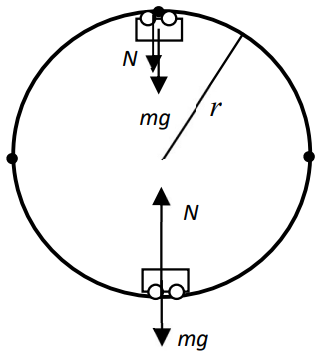
\includegraphics[scale=.5]{assets/rollercoaster.png}
	\caption{Rollercoaster on vertical circular track}
\end{marginfigure}
\begin{example}{}{rollercoaster}
	A rollercoaster of mass \(m\) moves along a vertical circular track of radius \(r\).
	At the top of the track, both \(mg\) and \(N_\text{top}\) act downwards to provide the centripetal acceleration.
	\[ma_c = N_\text{top} + mg\]
	At the top of the track, the minimum speed \(v_\text{min}\) occurs when \(N_\text{top}=0\).
	\[v_\text{min} = \sqrt{rg}\]

	At the bottom of the track, \(mg\) still acts downwards, but \(N_\text{bottom}\) acts upwards.
	\[ma_c = N_\text{bottom} - mg\]
\end{example}

\chapter{Oscillations}
\section{Free oscillations}
\begin{definition}{Simple harmonic motion}{shm}
	Oscillatory motion in which the \it{acceleration}
	\begin{itemize}
		\item is directly proportional to the displacement from the equilibrium position,
		\item is in the opposite direction to the displacement.
	\end{itemize}
	\begin{align*}
		a      & = -\omega^2 x          \\
		\omega & = 2\pi f = \f{2\pi}{T}
	\end{align*}
\end{definition}

\begin{marginfigure}
	\centering
	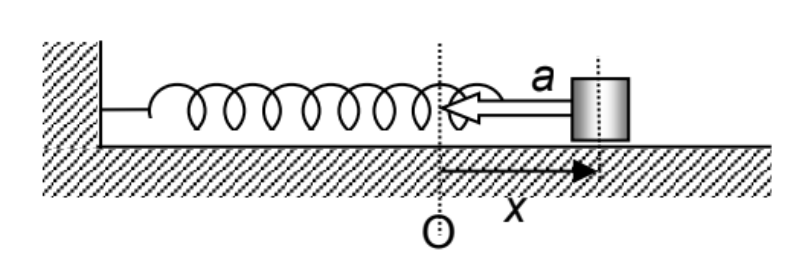
\includegraphics[scale=.4]{assets/mass-spring.png}
	\caption{Mass-spring system}
	\label{fig:mass-spring}
\end{marginfigure}
For a mass-spring system \cref{fig:mass-spring}, the elastic spring force acting on the mass
provides the restoring force, so
\begin{equation*}
	ma = -kx \implies a = -\f{k}{m}x\quad\ab(\omega = \sqrt{\lf{k}{m}})
\end{equation*}

\begin{marginfigure}
	\centering
	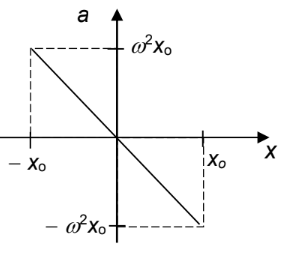
\includegraphics[scale=.7]{assets/shm-ax.png}
	\caption{\(a\) versus \(x\) gives a straight line}
	\label{fig:shm-ax}
\end{marginfigure}
Setting initial conditions as \(x(0) = 0\) and \(v(0) = v_0\), we can get \cref{tab:shm}.
\begin{table}[htpb]
	\centering
	\label{tab:shm}
	\begin{tabular}{c c c}
		\toprule
		qty             & maximum value          & equation                                                     \\
		\midrule
		\(x\)           & \(x_0\)                & \(x = x_0\sin\omega t\)                                      \\
		\(v = \dot{x}\) & \(v_0 = \omega x_0\)   & \(v = \omega x_0\cos\omega t = \pm\omega\sqrt{x_0^2 - x^2}\) \\
		\(a = \dot{v}\) & \(a_0 = \omega^2 x_0\) & \(a = -\omega^2 x_0\sin\omega t\)                            \\
		\bottomrule
	\end{tabular}
	\caption{Equations of s.h.m.}
\end{table}
\begin{marginfigure}
	\centering
	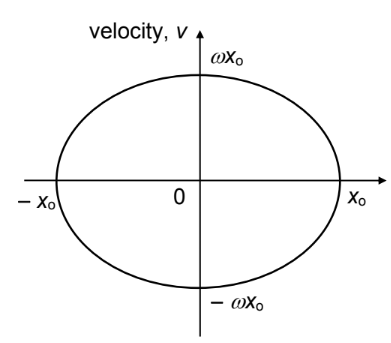
\includegraphics[scale=.6]{assets/shm-vx.png}
	\caption{\(v\) versus \(x\) gives an ellipse}
	\label{fig:shm-vx}
\end{marginfigure}

We can also derive
\begin{align*}
	E_\text{tot} = \max E_k & = \f{1}{2}m{v_0}^2 = \f{1}{2}m\omega^2 {x_0}^2                  \\
	E_k                     & = \f{1}{2}mv^2 = \f{1}{2}m\omega^2 {x_0}^2 \cos^2\omega t       \\
	E_p                     & = E_\text{tot} - E_k = \f{1}{2}m\omega^2 {x_0}^2 \sin^2\omega t
\end{align*}

Between oscillations of the same frequency, the phase difference is
\begin{equation*}
	\Delta\phi = \f{2\pi\Delta t}{T}
\end{equation*}
where \(\Delta t\) is the difference in time to reach the maximum displacement.
Oscillations \bf{in phase} have \(\Delta\phi = 0, 2\pi\), while those \bf{in antiphase} have \(\Delta\phi = \pi\).

\section{Damped oscillations}
\begin{definition}{Damped oscillations}{damped}
	Oscillatory motion in which \it{dissipative forces} cause a progressive decrease in amplitude.
\end{definition}
\begin{figure}[htpb]
	\centering
	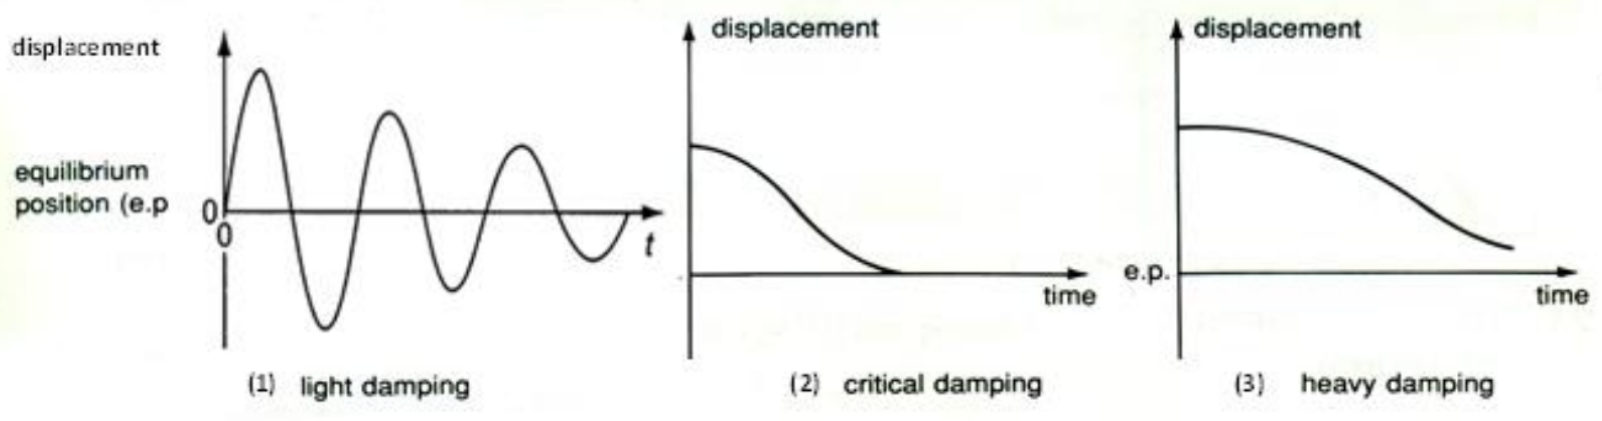
\includegraphics[width=1.1\textwidth]{assets/damping-types.png}
	\caption{Damped oscillations}
	\label{fig:damped}
\end{figure}
\begin{itemize}
	\item \bf{Light damping} causes the amplitude to \it{decrease exponentially with time} across \it{several oscillations} with \it{constant period}.
	\item \bf{Critical damping} causes the system to return to the eq.~pos.~in the shortest possible time without oscillating.
	\item \bf{Heavy damping} or \bf{overdamping} makes the system return to the eq.~pos.~in an infinitely long time.
\end{itemize}

\section{Forced oscillations}
\begin{definition}{Forced oscillations}{forced}
	Oscillatory motion in which an \it{external periodic driving force} is applied to the system.
\end{definition}
\begin{definition}{Resonance}{resonance}
	When the frequency of the external periodic driving force equals the \it{natural frequency} of the system,
	the amplitude of oscillations reaches a maximum.

	This frequency is also the \it{resonant frequency}.
\end{definition}
\begin{marginfigure}
	\centering
	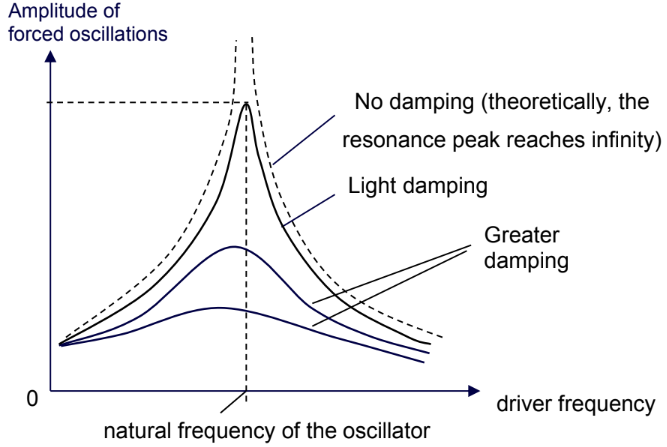
\includegraphics[width=\textwidth]{assets/damped-resonance.png}
	\caption{Resonance in damped system}
	\label{fig:damped-resonance}
\end{marginfigure}

\chapter{Waves}
Wave \bf{speed} \(v\) is the distance the wave profile travels per unit time, given by
\begin{equation*}
	v = f\lambda = \f{\lambda}{T}
\end{equation*}
\begin{itemize}
	\item \(f\) is the \bf{frequency}, the number of oscillations per unit time
	\item \(\lambda\) is the \bf{wavelength}, the distance between two adjacent points oscillating in phase
	\item \(T\) is the \bf{period}, the time taken for a point on the wave to complete one oscillation
\end{itemize}

\section{Progressive waves}
\begin{definition}{Progressive wave}{wave}
	A disturbance that propagates, carrying energy without physically transferring wave particles.
\end{definition}

\subsection{Wave graphs}
\begin{figure}[htpb]
	\centering
	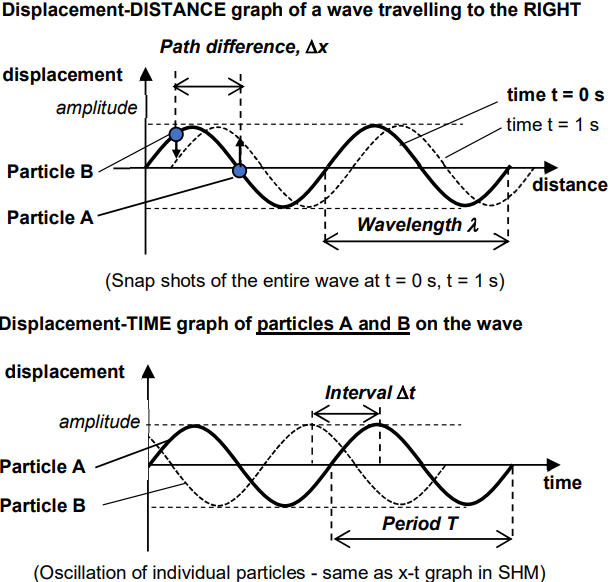
\includegraphics[width=\textwidth]{assets/wave-graphs.png}
	\caption{Wave graphs}
	\label{fig:wave-graphs}
\end{figure}

\bf{Displacement-distance graphs} take a `snapshot' of the wave at a particular instant \(\implies\) get \(\lambda\).
\it{Translate} the graph to get the wave profile at a later instant and find each point's direction of travel.
\[\Delta\phi = 2\pi\f{\Delta x}{\lambda}\]

\bf{Displacement-time graphs} show how one point on the wave oscillates with time \(\implies\) get \(T\).
The gradient \(\odv{y}{t}\) gives the speed of the point: \num{0} at the amplitude, extreme at the eq.~pos.
\[\Delta\phi = 2\pi\f{\Delta t}{T}\]

\subsection{Wave energy and intensity}
\begin{definition}{Intensity}{intensity}
	Rate at which energy is transported by the wave \it{per unit area} across
	a surface normal to direction of energy transfer. [\unit{\watt\per\square\meter}]
	\[\text{intensity} = \f{\text{power}}{\text{area}}\]
\end{definition}
Because \(E = \f{1}{2}m\omega^2{x_0}^2\),
\begin{align*}
	\text{energy}    & \propto \text{amplitude}^2 \\
	\text{intensity} & \propto \text{amplitude}^2
\end{align*}
For a wave from a \bf{point source},
\begin{align*}
	\text{intensity} & = \f{\text{power}}{\text{area}} = \f{P}{4\pi r^2} \\
	                 & \propto \lf{1}{r^2}
\end{align*}



\subsection{Transverse waves}
\begin{definition}{Transverse wave}{transverse}
	A \bf{transverse wave} is one in which points of disturbance oscillate about their eq.~pos.~\it{perpendicular}
	to the direction of energy propagation.
\end{definition}

\bf{EM waves} are transverse waves made up of mutually perpendicular \(\va{E}\) and \(\va{B}\) fields
perpendicular to the direction of energy propagation.
\begin{itemize}
	\item EM waves do not need a propagation medium; they \it{can propagate through vacuums}.
	\item EM waves travel at \(c = \qty{3.00e8}{\meter\per\second}\) in a vacuum.
\end{itemize}
\begin{table}[htpb]
	\centering
	\begin{tabular}{l l}
		\toprule
		type               & approximate \(\lambda\)              \\
		\midrule
		\bf{g}amma         & \(\qty{1e-15}{\meter}\)              \\
		\bf{x}-ray         & \(\qty{1e-10}{\meter}\)              \\
		\bf{u}ltraviolet   & \(\qty{1e-8}{\meter}\)               \\
		\bf{v}isible light & \(\qtyrange{400}{700}{\nano\meter}\) \\
		\bf{i}nfrared      & \(\qtyrange{0.7}{1}{\milli\meter}\)  \\
		\bf{m}icrowave     & \(\qty{1e-2}{\meter}\)               \\
		\bf{r}adio         & \(\qty{1e0}{\meter}\)                \\
		\bottomrule
	\end{tabular}
	\caption{EM spectrum}
	\label{tab:em-waves}
\end{table}

\begin{definition}{Polarisation}{polarisation}
	The phenomenon where vibrations in a transverse wave are \it{restricted to one direction},
	normal to the direction of energy transfer.
\end{definition}
\begin{marginfigure}
	\centering
	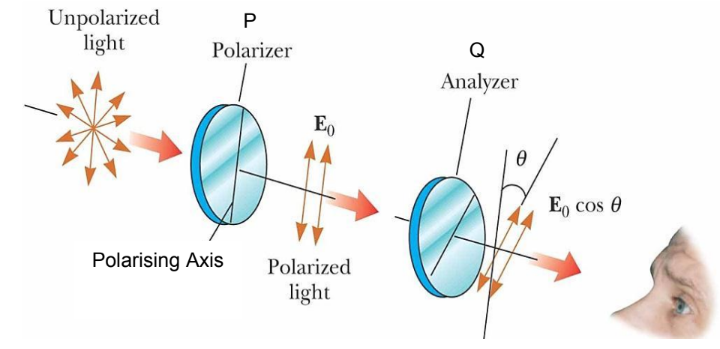
\includegraphics[width=\textwidth]{assets/polarise.png}
	\caption{Polarisation of light}
	\label{fig:polarise}
\end{marginfigure}
For a wave passing through two polarisers with an angle \(\theta\) between them\sidenote{The first polariser only allows vibrations parallel to its normal},
\[I_\text{result} = I_0 \cos^2\theta\]

\subsection{Longitudinal waves}
\begin{definition}{Longitudinal wave}{longitudinal}
	A \bf{longitudinal wave} is one in which points of disturbance oscillate about their eq.~pos.~\it{parallel}
	to the direction of energy propagation.
\end{definition}
At points where \(\text{displacement} = y = 0\),
\begin{itemize}
	\item \bf{compressions}	are regions where particles are closest together; particles before it have \(+y\) and particles after have \(-y\).
	\item \bf{rarefactions}	are regions where particles are furthest apart; particles before it have \(-y\) and particles after have \(+y\).
\end{itemize}

\chapter{Superposition}
\section{Principles}
\begin{definition}{Principle of superposition}{posoup}
	When 2 or more waves \it{of the same kind} overlap, the resultant displacement
	at any point equals the \it{vector sum} of the \it{individual displacements}
	at that point.
\end{definition}

\begin{definition}{Interference}{interference}
	The phenomenon where 2 or more waves superpose to form a resultant wave,
	whose amplitude is given by the Principle of Superposition.
\end{definition}

\begin{definition}{Coherence}{coherent}
	Coherent wave sources are those who maintain a \it{constant phase difference}
	between them.
\end{definition}

An interference pattern is \bf{observable} iff
\begin{enumerate}
	\item sources are \it{coherent}
	\item waves are approximately the same amplitude
	\item transverse waves are unpolarised or share the same polarisation direction
\end{enumerate}

\bf{Constructive interference} when two waves meet \it{in phase} \(\implies\) maximum resultant amplitude, maximum intensity.
\bf{Destructive interference} when two waves meet \it{in anti-phase} \(\implies\) minimum resultant amplitude, minimum intensity.

For two waves of the same amplitude \(A\),
\begin{table}[htpb]
	\centering
	\begin{tabular}{r c c}
		\toprule
		\hil{\bf{sources in phase}}                  & constructive                 & destructive                  \\
		\midrule
		amplitude \(A_\text{res}\)                   & \(2A\)                       & \(0\)                        \\
		intensity \(I_\text{res}\)                   & max                          & min                          \\
		path diff.~\(\delta\)                        & \(n\lambda\)                 & \(\f{1}{2}\ab(2n+1)\lambda\) \\
		phase diff.~\(\Delta\phi\)                   & \(2k\pi\)                    & \(\ab(2k+1)\pi\)             \\
		\toprule
		\hil[jiyoyellow]{\bf{sources in anti-phase}} & constructive                 & destructive                  \\
		\midrule
		amplitude \(A_\text{res}\)                   & \(0\)                        & \(2A\)                       \\
		intensity \(I_\text{res}\)                   & min                          & max                          \\
		path diff.~\(\delta\)                        & \(\f{1}{2}\ab(2n+1)\lambda\) & \(n\lambda\)                 \\
		phase diff.~\(\Delta\phi\)                   & \(\ab(2k+1)\pi\)             & \(2k\pi\)                    \\
		\bottomrule
	\end{tabular}
	\caption{Constructive and destructive interference}
	\label{tab:interference-types}
\end{table}

\section{Double slit}
For a double slit with distance between slits \(d\), distance
of slits to screen \(L\) and incident light of wavelength \(\lambda\).
\begin{figure}[htpb]
	\centering
	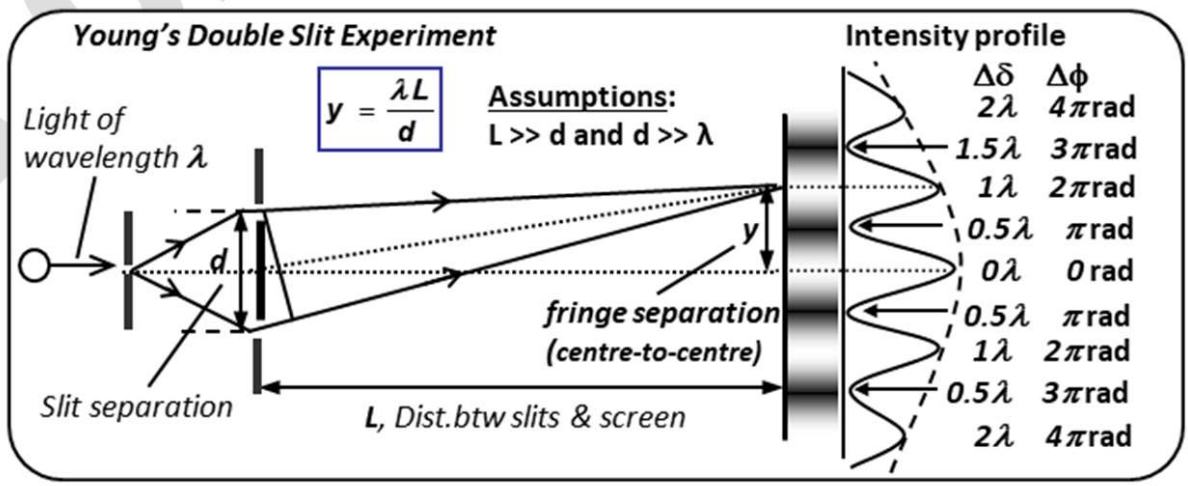
\includegraphics[width=\textwidth]{assets/double-slit.png}
	\caption{Double slit}
	\label{fig:double-slit}
\end{figure}

\it{Where can we find maxima/minima?} At angles \(\theta\), where
\begin{itemize}
	\item maxima (constructive): \(d\sin\theta=m\lambda\), where \(m \in \integers_0\)
	\item minima (destructive): \(d\sin\theta=(m-\num{0.5})\lambda\), where \(m \in \integers\)
\end{itemize}

Slits are separated by a \bf{slit separation} \(\Delta y\) where
\[\Delta y=\f{\lambda L}{d}\]

The assumption is that \(L\gg d\) and \(d \gg \lambda\).

\section{Diffraction grating}
For a diffraction grating with \(\lf{1}{d}\) slits per unit length (\(d\) is the slit spacing),
and incident light of wavelength \(\lambda\),
\[d\sin\theta=n\lambda\]
where \(n\) is the order.
\begin{figure}[htpb]
	\centering
	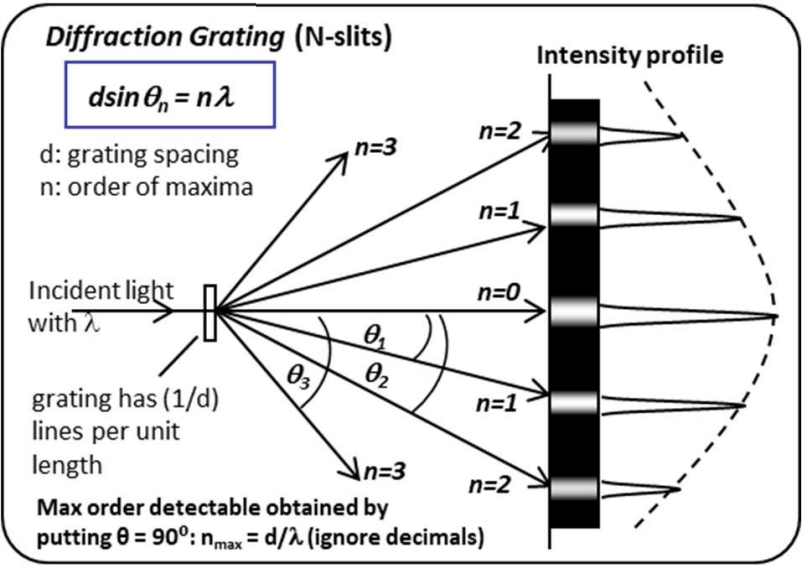
\includegraphics[width=0.75\textwidth]{assets/diffraction-grating.png}
	\caption{Diffraction grating}
	\label{fig:diffraction-grating}
\end{figure}


\section{Single slit diffraction}
\begin{marginfigure}
	\centering
	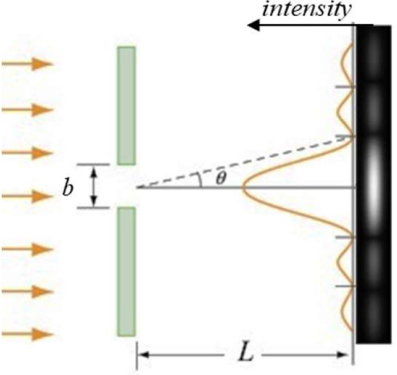
\includegraphics[width=\textwidth]{assets/single-slit.png}
	\caption{Single slit}
	\label{fig:single-slit}
\end{marginfigure}
With a single slit of width \(b\) and incident light of wavelength \(\lambda\),
the \bf{first minimum intensity} is at \(\theta\) where
\[\sin\theta=\f{\lambda}{b}\]

\begin{definition}{Rayleigh criterion}{rayleigh}
	Two images are \it{just resolvable} when the centre of one image's
	diffraction pattern is \it{directly over} the first minimum of the other's diffraction pattern.
\end{definition}
\begin{marginfigure}
	\centering
	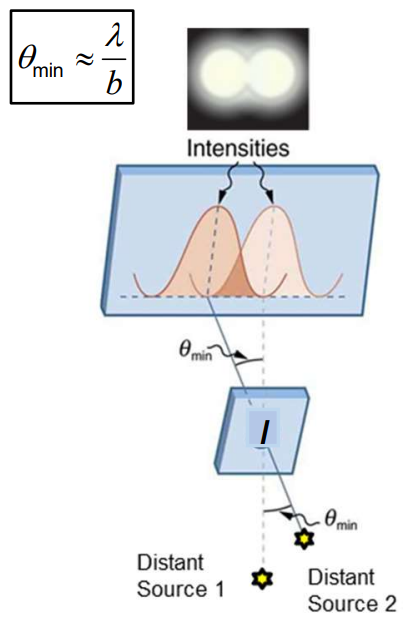
\includegraphics[width=.8\textwidth]{assets/rayleigh.png}
	\caption{Rayleigh criterion}
	\label{fig:rayleigh}
\end{marginfigure}
The aperture's \bf{resolving power} is then
\[\theta_{\min} \approx \f{\lambda}{b}\]

\section{Stationary waves}
\begin{marginfigure}
	\centering
	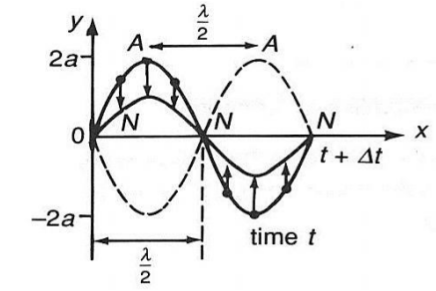
\includegraphics[width=\textwidth]{assets/stationary-wave.png}
	\caption{Stationary wave \(y\) versus \(x\)}
	\label{fig:stationary-waves}
\end{marginfigure}
\begin{definition}{Stationary waves}{stationary-waves}
	are formed when two similar waves of the \it{same frequency},
	\it{same speed}, and \it{same amplitude} \(A\) travel in
	\it{opposite directions} and superpose.
\end{definition}
\begin{itemize}
	\item \bf{Antinodes} are where amplitude is a maximum (\(2A\));
	      \bf{nodes} are where amplitude is a minimum (\num{0}).
	\item Particles in the same segment are in phase; particles in adjacent segments are in antiphase.
	\item Wavelength \(\lambda = 2\cdot\text{distance from A to A}\)
	\item Energy is not propagated.
\end{itemize}

\subsection{String fixed at two ends}
Where \(L\) is the string's length, the frequency and wavelength at the \(n\)th harmonic are
\begin{align*}
	f_n       & = n\f{v}{2L} \\
	\lambda_n & = \f{2L}{n}
\end{align*}

\subsection{Air columns}
Air columns come in closed pipes and open pipes.
\begin{table}[htpb]
	\centering
	\begin{tabular}{r l l}
		\toprule
		               & closed pipe                                      & open pipe                \\
		\midrule
		disp.~A/N      & disp.~N at closed end, disp.~A at open end       & both ends disp.~A        \\
		pressure A/N   & pressure A at closed end, pressure N at open end & both ends pressure N     \\
		\(f_n\)        & \(\lf{nv}{4L},\:n=2k+1\)                         & \(\lf{nv}{2L}\)          \\
		\(\lambda_n\)  & \(\lf{4L}{n},\:n=2k+1\)                          & \(\lf{2L}{n}\)           \\
		end correction & \(\lf{\lambda}{4}=L+c\)                          & \(\lf{\lambda}{2}=L+2c\) \\
		\bottomrule
	\end{tabular}
	\label{tab:closed-open-pipes}
	\caption{Closed and open pipes}
\end{table}

\chapter{Gravitation}
\section{F and g}

\begin{definition}{Newton's Law of Universal Gravitation}{nlug}
	Every \it{point mass} attracts every other point mass with a force
	\begin{enumerate}
		\item directly proportional to the product of their masses
		\item inversely proportional to the square of the distance between them
	\end{enumerate}
	\[F = \f{GMm}{r^2} = -\odv{U}{r}\]
\end{definition}

\begin{definition}{Gravitational field strength}{grav-field}
	Gravitational force \it{per unit mass} acting on a small point mass
	placed at a point within a gravitational field
	\[g = \f{F}{m} = \f{G M}{r^2} = -\odv{\phi}{r}\]
\end{definition}

\bf{Gravitational field lines} are
\begin{itemize}
	\item \it{directed radially} towards a point mass
	\item \it{spreading out} at further distances from the point mass
\end{itemize}

\begin{example}{}{earth-g}
	The value of \(\va{g}\) varies at different points on Earth's surface, because
	\begin{itemize}
		\item the Earth is rotating
		\item the Earth is not a perfect sphere (bulges at the equator)
		\item the Earth's density is not uniform
	\end{itemize}
\end{example}

\begin{definition}{Weightlessness}{weightlessness}
	Sensation when \it{no physical contact force} acts on the body (e.g.~during free fall)
\end{definition}

\bf{Geostationary satellites} are those which
\begin{itemize}
	\item have a period of \qty{24}{\hour}
	\item have the same direction of rotation as the Earth (west to east)
	\item rotate in the plane containing the equator
\end{itemize}

\section{U and phi}
\begin{definition}{Gravitational potential energy}{gpe}
	Work done by an external force to bring a small test mass at infinity to
	a point within a gravitational field \it{with no change in k.e.}.
	\[U = -\f{GMm}{r} = \int^{r}_{\infty} \va{F} \odif{r}\]
\end{definition}

\begin{example}{}{negative-gpe}
	\it{Why is GPE negative?}
	\begin{itemize}
		\item \(\va{F}_g\) is attractive in nature
		\item To bring a mass from infinity to a point within a gravitational field, we must apply an external force \it{opposite} to \(\va{F}_g\)
		\item External force and mass's displacement are in \it{opposite directions} \(\implies\) the external force does \it{negative work}
	\end{itemize}
\end{example}

\begin{definition}{Gravitational potential}{grav-pot}
	Work done \it{per unit mass} by an external force to bring a small test mass
	from infinity to a point within a gravitational field, with \it{no change in k.e.}.
	\[\phi = \f{U}{m} = -\f{GM}{r} = \int^{r}_{\infty} \va{g} \odif{r}\]
\end{definition}
Moving a mass \(m\) from one point of potential \(\phi_i\) to another
point of potential \(\phi_f\) means that \(\Delta U = m\ab(\phi_f-\phi_i)\).
\term{The work done on the mass is \(W = -\Delta U\).}

\begin{marginfigure}
	\centering
	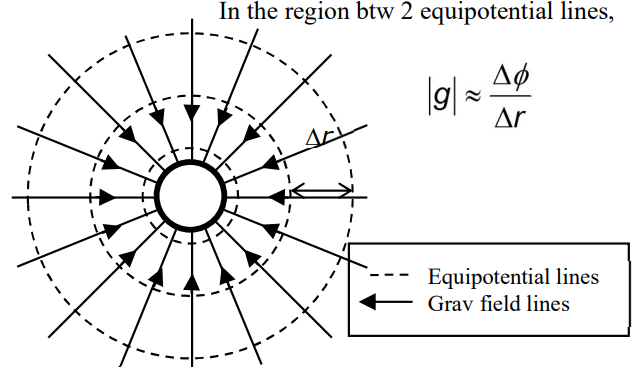
\includegraphics[width=\textwidth]{assets/g-phi.png}
	\label{fig:g-phi}
	\caption{\(g\) and equi-\(\phi\) lines}
\end{marginfigure}

\section{Other examples}
Let \(R \coloneq\) the radius of the Earth and \(M \coloneq\) its mass.
\begin{example}{Escape speed}{escape-speed}
	Projecting a mass \(m\) with an \bf{escape speed} \(v\) from the surface of the Earth
	will cause the mass to escape the Earth's \(g\)-field.
	For \(\min v\),
	\begin{align*}
		K_i + U_i                    & = K_f + U_f            \\
		\f{mv^2}{2}+\ab(-\f{GMm}{R}) & = 0                    \\
		\implies v                   & = \sqrt{\frac{2GM}{R}}
	\end{align*}
\end{example}

\begin{example}{Orbiting satellite}{orbiting-satellite}
	A satellite of mass \(m\) orbiting the Earth at a distance \(r\) from its centre
	with speed \(v\) will need gravitational force to provide its centripetal
	acceleration (\(F_g\) provides \(F_c\)).
	\begin{align*}
		\f{mv^2}{r}              & = \f{GMm}{r^2}     \\
		v                        & = \sqrt{\f{GM}{r}} \\
		\implies K = \f{mv^2}{2} & = \f{GMm}{2r}
	\end{align*}

	Total energy isn't conserved when the satellite moves from
	an orbit radius \(r_i\) to a new orbit radius \(r_f\).
	\begin{align*}
		K_i + U_i + W_{\text{ext}}                          & = K_f + U_f                              \\
		\f{GMm}{2r_i} + \ab(-\f{GMm}{r_i}) + W_{\text{ext}} & = \f{GMm}{2r_f} + \ab(-\f{GMm}{r_f})     \\
		-\f{GMm}{2r_i} + W_{\text{ext}}                     & = -\f{GMm}{2r_f}                         \\
		W_{\text{ext}}                                      & = \f{GMm}{2}\ab(\f{1}{r_i} - \f{1}{r_f})
	\end{align*}
\end{example}

\begin{example}{Binary star}{binary-star}
	For two stars \(m_1\) and \(m_2\) orbiting at radii \(r_1\) and \(r_2\) about a common centre,
	\(F_g\) provides \(F_c\) of either star.
	\begin{align*}
		\f{Gm_1m_2}{\ab(r_1+r_2)^2} & = m_1r_1\omega^2 = m_2r_2\omega^2 \\
		\implies \lf{m_1}{m_2}      & = \lf{r_2}{r_1}
	\end{align*}
\end{example}

\begin{figure}[htpb]
	\centering
	\input{assets/g-summary.tikz}
	\caption{Formulae}
	\label{fig:g-summary}
\end{figure}


% j2 topic
\chapter{Thermal physics}
\section{Heat transfer}
\begin{definition}{Thermal equilibrium}{thermal-eq}
	The phenomenon in which two bodies in thermal contact
	have \it{no net exchange of heat} between them.
\end{definition}
\begin{definition}{0LoT}{0lot}
	If bodies A and B are \it{separately in thermal eq.}~with a third body
	C, then A and B are in thermal eq.~with each other.
\end{definition}
\begin{definition}{Heat capacities}{heat-capacity}
	\par
	\bf{Specific heat capacity} \(c\) is the amount of energy
	per unit mass required to cause an increase in one unit of temperature [\unit{\joule\per\kilogram\per\kelvin}].
	\[Q=mc\Delta T\]

	\bf{Heat capacity} \(C\) is the amount of energy
	required to cause an increase in one unit of temperature [\unit{\joule\per\kelvin}].
	\[Q=C\Delta T\]
\end{definition}
\begin{definition}{Latent heats}{latent-heat}
	\par
	\bf{Specific latent heat of fusion} \(l_f\) --- the amount of energy
	per unit mass required to change a substance \it{from solid to liquid} with no change in temperature [\unit{\joule\per\kilogram}].
	\[Q=ml_f\]

	\bf{Specific latent heat of vaporization} \(l_v\) --- the amount of energy
	per unit mass required to change a substance \it{from liquid to gas} with no change in temperature [\unit{\joule\per\kilogram}].
	\[Q=ml_v\]
\end{definition}

Solving problems involving heat transfer involve \term{energy conservation}.
\[\text{total heat loss} = \text{total heat gain}\]

\begin{example}{}{ct1-q7}
	A glass beaker (\(m_b = \qty{170}{\gram}\), \(c_b = \qty{0.84}{\joule\per\gram\per\kelvin}\))
	at \qty{28}{\celsius} contains \it{ice} (\(m_i = \qty{120}{\gram}\), \(c_i=\qty{2.05}{\joule\per\gram\per\kelvin}\))
	at \qty{-15}{\celsius} and boiling \it{water} (\(m_w = \qty{90}{\gram}\), \(c_w = \qty{4.18}{\joule\per\gram\per\kelvin}\)).

	When thermal equilibrium is reached, there is both water and ice in the beaker. No water evaporates.
	(\(l_f = \qty{334}{\joule\per\gram}\))

	\it{Find the mass of ice \({m_i}'\) that melts during this process.}
	\vspace*{5mm}

	deduction---
	\begin{center}
		`water and ice in the beaker' \(\implies\) final temperature is \qty{0}{\celsius} \\
		`thermal equilibrium reached' \(\implies\) heat lost = heat gained; final temperature is the same for all bodies
	\end{center}
	\vspace*{5mm}

	working---
	\begin{align*}
		\sum\text{heat loss}                  & = \sum\text{heat gain}                \\
		m_w c_w\ab(100-0)  + m_b c_b\ab(28-0) & = m_i c_i\ab(0-\ab(-15)) + {m_i}' l_f \\
		{m_i}'                                & = \qty{114}{\gram}
	\end{align*}
\end{example}

\section{Molecular view}
\begin{definition}{Internal energy}{internal-energy}
	The summation of:
	\begin{itemize}
		\item \it{microscopic kinetic energy} due to the molecules' random motion
		\item \it{microscopic potential energy} due to intermolecular forces
	\end{itemize}
	\[U = \sum E_k + \sum E_p\]
\end{definition}
\begin{definition}{Temperature}{temperature}
	A measure of the average kinetic energy of the molecules in a substance.
\end{definition}
\begin{table}[htpb]
	\centering
	\begin{tabular}{r c c}
		\toprule
		                        & \(E_k\)           & \(E_p\) \\
		\midrule
		phase change            & ---               & change  \\
		\(T\) increase/decrease & increase/decrease & ---     \\
		\bottomrule
	\end{tabular}
	\label{tab:ek-ep}
	\caption{What changes?}
\end{table}

\section{Ideal gases}
\begin{definition}{Ideal gas}{ideal-gas}
	A theoretical model of a gas which satisfies
	\[pV = nRT\]
	where \(p\) is the pressure, \(V\) is the volume, \(n\) is the number of moles, \(R\) is the ideal gas constant and \(T\) is the temperature.
\end{definition}
Ideal gas \bf{assumptions} include
\begin{itemize}
	\item A gas consists of a very large number of molecules
	\item The molecules are in constant random motion
	\item Gas molecules' collisions with one another and the container walls are perfectly elastic
	\item No intermolecular forces between gas molecules
	\item Volume of gas molecules is negligible compared to the volume of the container
	\item Duration of collisions is negligible compared to the time between collisions
\end{itemize}
\subsection{Pressure}
\begin{definition}{Gas pressure}{gas-pressure}
	The \it{average force per unit area} exerted by gas molecules on the container walls
\end{definition}
Pressure is due to number of molecules \(N\), molecule mass \(m\), molecule speed \(c\) and volume \(V\).

Assume a large number of molecules \(N\) in a cubical container of side \(s\).
For each molecule, resolve its velocity \(c_i\) in 3d; \({c_i}^2 = {u_i}^2 + {v_i}^2 + {w_i}^2\).

Choose any container wall. In the \(x\)-direction, a molecule colliding with the wall
will experience a change in momentum
\[\Delta p = p_f-p_i = -mu-\ab(+mu) = -2mu\]

The time taken for any collision \(\Delta t = \f{2s}{u}\), so the average force exerted
on the chosen wall by one molecule is
\[\ab<F> = \ab|\f{\Delta p}{\Delta t}| = \f{2mu\cdot u}{2s} = \f{mu^2}{s}\]

The total force exerted on the wall by all \(N\) molecules is
\[\sum F = N\ab<F> = \f{Nm\ab<u^2>}{s}\]

The total pressure exerted on the wall is the total force per unit area:
\[p = \f{\sum F}{s^2} = \f{Nm\ab<u^2>}{s^3} = \f{Nm\ab<u^2>}{V}\]

Given that \(\ab<c^2> = \ab<u^2> + \ab<v^2> + \ab<w^2>\), and
because all molecules are in constant random motion (with no preferred direction),
\[\ab<u^2> = \f{1}{3}\ab<c^2>\]
Thus
\begin{equation*}
	pV = \f{1}{3}Nm\ab<c^2>
\end{equation*}
\(\ab<c^2>\) is the mean square speed; \(\sqrt{\ab<c^2>}\) is the r.m.s.~speed.

\subsection{Temperature}
Derive:
\begin{align*}
	pV = \f{1}{3}Nm\ab<c^2>               & = NkT                        \\
	\implies \f{1}{2}m\ab<c^2>            & = \f{3}{2}kT                 \\
	\implies U =  N\cdot\f{1}{2}m\ab<c^2> & = \f{3}{2}NkT  = \f{3}{2}nRT \\
\end{align*}
The internal energy is directly proportional to the temperature (\(U\propto T\))\sidenote{assuming gas is monoatomic}; it is independent of the pressure and volume.

\section{State}
\begin{definition}{1LoT}{1lot}
	The increase in internal energy of a system is equal to
	the (1) \it{heat supplied to the system} plus the (2) \it{work done \bf{on the system}} by external forces.
	\[\Delta U = Q + W\]
	\small \[W = \int p\odif{V}\]
\end{definition}
\begin{table}[htpb]
	\centering
	\begin{tabular}{r c c}
		\toprule
		      & \(Q\)              & \(W\)            \\
		\midrule
		\(+\) & heat enters system & system contracts \\
		\(-\) & heat leaves system & system expands   \\
		\bottomrule
	\end{tabular}
	\label{tab:q-and-w}
	\caption{Signs of \(Q\) and \(W\)}
\end{table}

Some important thermodynamic processes\sidenote{we defined \(W\) as `work done on the system', so \(\Delta V>0\implies W<0\) and v.v.}:
\begin{table}[htpb]
	\centering
	\begin{tabular}{r l c c c}
		\toprule
		process       & involves         & \(Q =\)        & \(W=\)              & \(\Delta U=\) \\
		\midrule
		isothermal    & \(T\) constant   & \(-W\)         & \(-\int p\odif{V}\) & \(0\)         \\
		isovolumetric & \(V\) constant   & \(mc\Delta T\) & \(0\)               & \(Q\)         \\
		adiabatic     & no heat transfer & \(0\)          & \(-\int p\odif{V}\) & \(W\)         \\
		isobaric      & \(p\) constant   & \(mc\Delta T\) & \(-p\Delta V\)      & \(Q+W\)       \\
		\bottomrule
	\end{tabular}
	\caption{Thermodynamic processes}
	\label{tab:thermo-processes}
\end{table}

\begin{marginfigure}
	\centering
	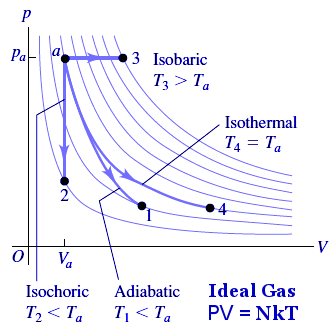
\includegraphics[width=\textwidth]{assets/thermo-processes.png}
	\caption{\(pV\) diagrams}
	\label{fig:pv-diagram}
\end{marginfigure}

\begin{definition}{Cyclic process}{cyclic-process}
	A process in which the system returns to its initial state at the end of the process.
	\[\Delta U = 0 \implies Q_\text{net} = -W_\text{net}\]
\end{definition}

\chapter{Electric field}
\section{E and F}
\begin{definition}{E-field, E-field strength}{efield}
	An electric field is a \it{region of space} where a charge experiences an
	electric force.

	Electric field strength \(E\) is the electric force per unit charge
	acting on a \it{positive charge} placed at a point.
	\[\va{E} = \f{\va{F}}{q} = -\odv{V}{r}\]
\end{definition}
\(E\) within a conductor equals \(0\).

\(\va{E}\)-field lines
\begin{itemize}
	\item direct from higher potential (more positive) to lower potential (more negative)
	\item are proportional to the magnitude of the charge
	\item do not intersect
\end{itemize}
\begin{figure}[htpb]
	\centering
	\begin{minipage}{.32\textwidth}
		\centering
		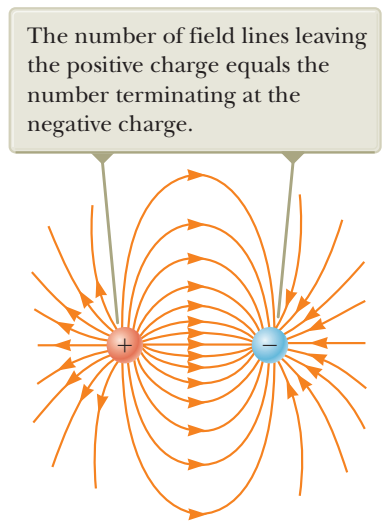
\includegraphics[width=.97\textwidth]{assets/q-minus-q.png}
		\caption{two opposite point charges}
	\end{minipage}
	\begin{minipage}{.32\textwidth}
		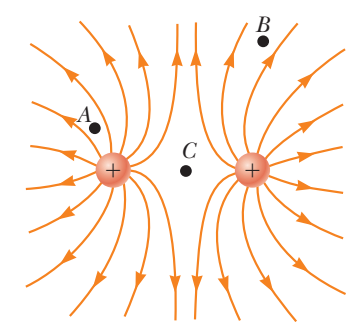
\includegraphics[width=.97\textwidth]{assets/q-q.png}
		\caption{two positive point charges}
	\end{minipage}
	\begin{minipage}{.32\textwidth}
		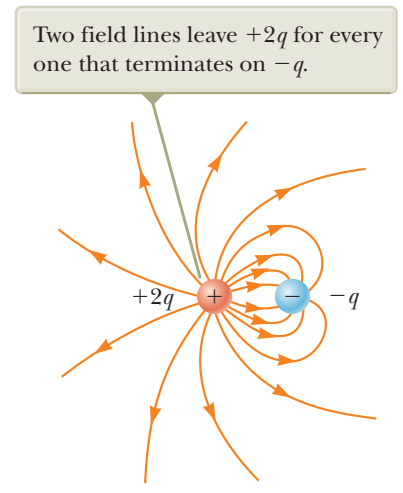
\includegraphics[width=.97\textwidth]{assets/2q-minus-q.png}
		\caption{two opposite point charges \(+2q\) and \(-q\)}
	\end{minipage}
\end{figure}

\begin{definition}{Coulomb's law}{eforce}
	Magnitude of the electric force between two point charges is
	\begin{enumerate}
		\item directly proportional to the product of the magnitude of the charges
		\item inversely proportional to the square of the distance between them
	\end{enumerate}
	\[F = \f{q_1q_2}{4\pi\epsilon_0r^2}=-\odv{U}{r}\]
	\(\epsilon_0 = \) permittivity of free space
\end{definition}

\section{U and V}
\begin{definition}{Electric potential energy}{epe}
	Work done by an external force in assembling a system of charges
	\it{originally at infinity}, with \it{no change in k.e.}
	\begin{align*}
		U                        & = \f{q_1q_2}{4\pi\epsilon_0r}  \\
		U\text{ (by ext. force)} & = U\text{ (by electric force)}
	\end{align*}
	for multiple charges, \(U = \sum_{\forall i,j}U_{ij}\)
\end{definition}
\begin{definition}{Electric potential}{epotential}
	Work done \it{per unit charge} by an ext.~force in bringing a small positive test charge
	from infinity to a point within an electric field, with \it{no change in k.e.}
	\begin{align*}
		V & = \f{U}{q} = \f{q}{4\pi\epsilon_0r}
	\end{align*}
\end{definition}
The change in potential energy\sidenote{work done by \bf{ext.~agent}!} in moving a charge from a
point of potential \(V_i\) to another point of potential \(V_f\) is \(\Delta U = q\ab(V_f - V_i)\).

\(V\) within a conductor is constant.

\bf{Equipotential lines}
\begin{itemize}
	\item distance between lines \(\propto\) \(\va{E}\)-field strength
	\item are perpendicular to \(\va{E}\)-field lines
\end{itemize}
\begin{figure}[htpb]
	\centering
	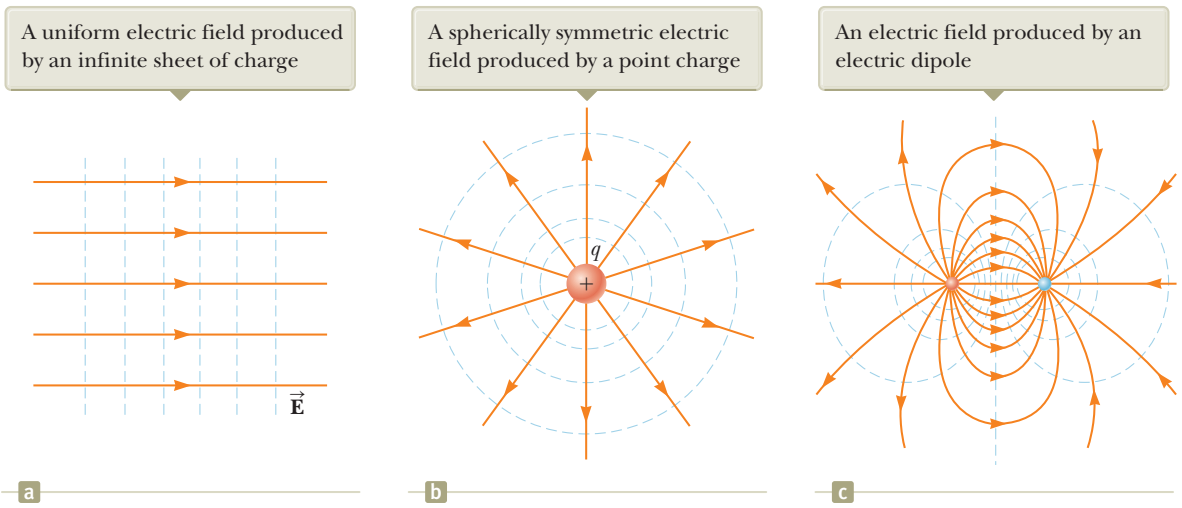
\includegraphics[width=.9\textwidth]{assets/v-lines.png}
	\caption{Equipotential lines and \(\va{E}\)-field lines}
	\label{fig:v-lines}
\end{figure}

A \bf{uniform electric field} is one where the \(\va{E}\)-field strength is the same at all points.
For a potential difference \(V\) applied across a distance \(d\),
\[E = \f{V}{d}\]
\begin{marginfigure}
	\centering
	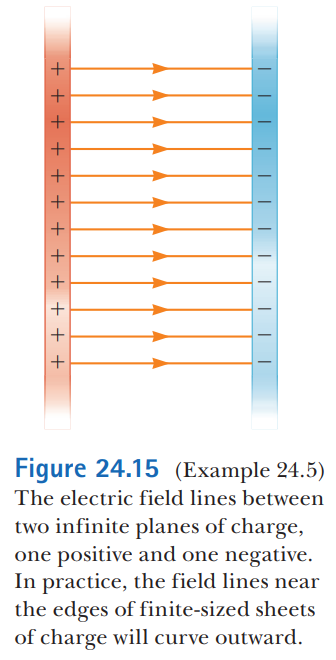
\includegraphics[width=.5\textwidth]{assets/uniform-efield.png}
	\caption{Uniform electric field}
	\label{fig:uniform-efield}
\end{marginfigure}

\begin{marginfigure}
	\centering
	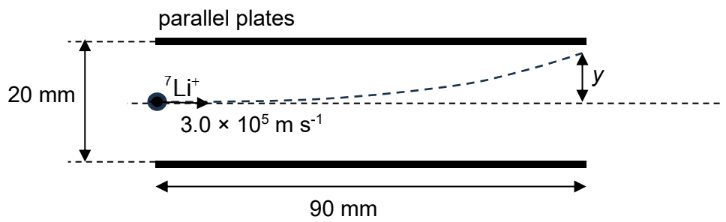
\includegraphics[width=.9\textwidth]{assets/accelerating-li.png}
	\caption{Accelerating \ce{Li+} ion}
	\label{fig:accel-li}
\end{marginfigure}
\begin{example}{}{accelerating-charge}
	\Cref{fig:accel-li} where a \ce{^7Li+} ion (\(m\), \(q\)) is accelerated with a initial
	horizontal velocity \(\va{u}\) through an electric field created by a
	potential difference \(V\) applied over two charged plates of length \(L\),
	separated by distance \(d\). \it{What is the vertical deflection \(y\) of the ion?}

	Since there are no ext.~forces, energy is conserved. We can use the kinematic equations.
	By N2L, \(ma = qE \implies a = \lf{qE}{m} = \lf{qV}{md}\).
	\begin{align*}
		y & = u_yt + \f{1}{2}a_yt^2                 \\
		  & = 0 + \f{1}{2}\f{qV}{md}\ab(\f{L}{u})^2 \\
		  & = \f{qL^2V}{2mdu^2}
	\end{align*}
\end{example}

\section{Summary}
\begin{figure}[htpb]
	\centering
	\input{assets/e-summary.tikz}
	\caption{Summary of electric field}
	\label{fig:e-summary}
\end{figure}

\chapter{Currents and circuits}
\section{Current}
\begin{definition}{Current}{current}
	Rate of flow of electric charge.
	\[I = \odv{q}{t} = \f{q_\text{tot}}{\Delta t}\:\text{for const.~current}\]
\end{definition}
Conventional current flows in the same direction as \hil{positive charges}.

The current flowing through a \bf{conductor} is
\[I = nAvq\]
\begin{itemize}
	\item \(n\) is the number of mobile charge carriers per unit volume\sidenote{intrinsic to the material}---number density [\unit{\per\cubic\metre}]
	\item \(A\) is the cross-sectional area
	\item \(v\) is drift velocity of charge carriers\sidenote{for the same material, \(v\propto\lf{1}{A}\)}
	\item \(q\) is the charge of one charge carrier
\end{itemize}

\section{V and emf}
\begin{definition}{Electromotive force}{emf}
	Energy converted \it{per unit charge} to electrical energy
	in driving charge around a complete circuit.
	\[\epsilon = \lf{W}{q}\]
\end{definition}
Emf is provided by an \hil{emf source} (e.g.~battery, generator),
where other forms of energy \(\to\) electrical energy.

\begin{definition}{Potential difference}{pd}
	Between two points, \underline{p.d.}~\(=\)~energy converted per unit
	charge from electrical energy \(\to\) other forms of energy,
	when charge is moved between the two points.
	\[\Delta V = \f{W}{q}\]
\end{definition}
P.d.~exists between two points/components in a circuit, where
electrical energy \(\to\) other forms of energy.

\section{Resistance}
\begin{definition}{Resistance}{resistance}
	\underline{Ratio} of p.d.~across a component to the current flowing through it. [\(\qty{1}{\ohm}=\qty{1}{\volt\per\ampere}\)]
	\[R = \f{V}{I} \neq \odv{V}{I}\]
	Not the gradient of a \(V\)-\(I\) graph.
\end{definition}

In circuits, \hil{effective resistance} is
\begin{align*}
	R_\text{eff} & = \sum_i R_i \quad\text{resistors \hil{in series}}                    \\
	R_\text{eff} & = \ab(\sum_i \f{1}{R_i})^{-1} \quad\text{resistors \hil{in parallel}}
\end{align*}

\begin{definition}{Ohm's law}{ohms-law}
	Provided that temperature/other physical conditions are constant,
	through a \it{metallic conductor},
	current flowing through it is directly proportional to the p.d.~across it.
\end{definition}

For a conductor of length \(L\), cross-sectional area \(A\), and resistivity\sidenote{intrinsic to the material} \(\rho\),
\[R = \f{\rho L}{A}\]

\section{Power}
\begin{definition}{Power}{e-power}
	Rate at which energy is converted from one form to another in a device
	\[P = IV \quad \text{(for all kinds of components)}\]
\end{definition}
For devices that \it{dissipate heat} (e.g.~resistors),
\[P = IV = I^2 R = \f{V^2}{R}\]

In practical applications, appliances should have \hil{high voltages}
so that the current is low (to produce the same power output).
Power loss due to Joule heating \(I^2R\) will be reduced.

\section{Circuits}
\subsection{\(I\)-\(V\) characteristics}
\begin{table}[htpb]
	\centering
	\begin{tabular}{r c l}
		\toprule
		component          & symbol                            & resistance...                                     \\
		\midrule
		metallic conductor & \tikz\draw(0,0) to[R] (1.5,0);    & is constant (\cref{def:ohms-law})                 \\
		filament lamp      & \tikz\draw(0,0) to[lamp] (1.5,0); & increases with temperature                        \\
		thermistor         & \tikz\draw(0,0) to[thR] (1.5,0);  & decreases with temperature                        \\
		diode              & \tikz\draw(0,0) to[Do] (1.5,0);   & forward biased: small; reverse biased: very large \\
		\bottomrule
	\end{tabular}
	\caption{Resistance of common components}
	\label{tab:component-resistance}
\end{table}
The components in \cref{tab:component-resistance} have various \(I\)-\(V\) characteristics (\term{memorise!}).
\begin{figure}[htpb]
	\centering
	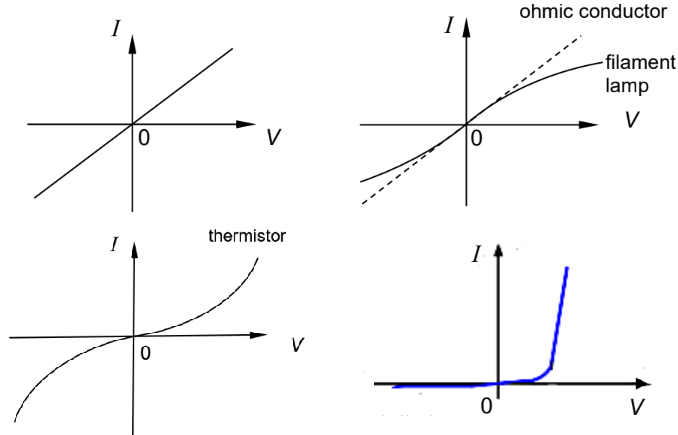
\includegraphics[width=0.8\textwidth]{assets/iv-characteristics.png}
	\caption{Some \(I\)-\(V\) characteristics}
	\label{fig:iv-characteristics}
\end{figure}
Explanations for common components
\begin{itemize}
	\item \bf{ohmic conductor} --- when \(T\) const, amplitude of lattice ion vibrations const. \(v\) const, \(R\) const.
	\item \bf{filament lamp}
	      \begin{itemize}
		      \item larger p.d., \(T\) increase.
		      \item amplitude of lattice ion vibrations increase, \(v\) decrease (given no change in \(n\)), \(R\) increase.
	      \end{itemize}
	\item \bf{thermistor} (negative temp.~coeff.)
	      \begin{itemize}
		      \item larger p.d., \(T\) increase
		      \item lattice vibrations increase, so hindrance to charge carrier flow increases (\(v\) decrease)
		      \item \it{but} thermistor also releases more charge carriers (\(n\) increase)
		      \item increase in \(n\) \it{larger than} the decrease in \(v\)
		      \item ratio \(\lf{V}{I}\) decrease, \(R\) decrease
	      \end{itemize}
	\item \bf{semiconductor diode} --- overly high reverse-biased p.d.~causes breakdown
\end{itemize}

\subsection{Internal resistance}
Emf sources have internal resistances \(r\), \cref{fig:int-resistance}.
\begin{marginfigure}
	\centering
	\begin{circuitikz}[scale=.8]
		\draw (0,0) to[R=$R$,v=$V_R$,i=$I$] (6, 0) -- (6,2) to[R=$r$] (3,2) to[battery1, l=\(\epsilon\), invert] (2,2) -- (0,2) -- (0, 0);
	\end{circuitikz}
	\caption{Internal resistance}
	\label{fig:int-resistance}
\end{marginfigure}
\begin{align*}
	\epsilon & = V_R + V_r   \\
	         & = I\ab(R + r) \\
	         & = V_R + Ir
\end{align*}

\subsection{Potential divider}
The p.d.~across any component is proportional to its resistance, within
the same closed loop.
\begin{marginfigure}
	\centering
	\begin{circuitikz}[scale=.8]
		\draw (6,2) to[battery1, l=$\epsilon$, invert] (0,2) to[short, -*, i=$I$] (0, 0) to[R=$R_1$, v=$V_1$] (2.5,0) to[short, -*, i=$I$] (3,0) to[R=$R_2$, v=$V_2$, i=$I$] (5.5,0) to[short,-*] (6,0) -- (6,2);
	\end{circuitikz}
	\caption{Potential divider}
	\label{fig:v-divider}
\end{marginfigure}
\begin{align*}
	I   & = \f{\epsilon}{R_1 + R_2}           \\
	V_1 & = IR_1 = \f{R_1}{R_1 + R_2}\epsilon \\
	V_2 & = IR_2 = \f{R_2}{R_1 + R_2}\epsilon \\
\end{align*}

\begin{marginfigure}
	\centering
	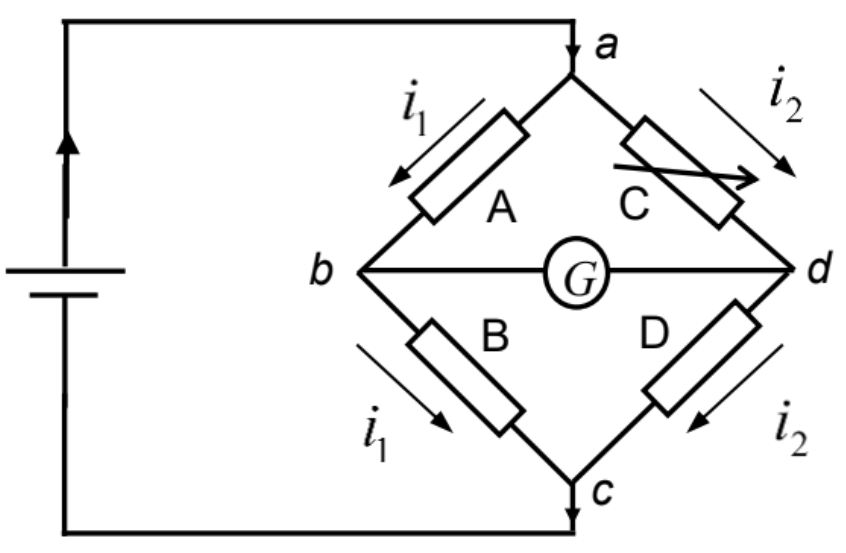
\includegraphics[width=\textwidth]{assets/wheatstone.png}
	\caption{Wheatstone bridge}
	\label{fig:wheatstone}
\end{marginfigure}
\begin{example}{}{wheatstone}
	The Wheatstone bridge (\cref{fig:wheatstone}) is useful for determining an unknown resistance \(R_C\).
	\begin{align*}
		V_{ab}                    & = V_{ad}        \\
		\implies i_1R_A           & = i_2R_C        \\
		V_{bc}                    & = V_{dc}        \\
		\implies i_1R_B           & = i_2R_D        \\
		\therefore\;\lf{R_A}{R_B} & = \lf{R_C}{R_D}
	\end{align*}
\end{example}

\section{Capacitors}
\begin{definition}{Capacitance}{capacitance}
	The ratio of the magnitude of the charge \(q\) to the potential difference across
	a capacitor \(V\). [\(\qty{1}{\farad} = \qty{1}{\coulomb\per\volt}\)]
	\[C = \f{q}{V}\]
\end{definition}
\hil{Effective capacitance} is
\begin{align*}
	C_\text{eff} & = \ab(\sum_i \f{1}{C_i})^{-1} \quad\text{capacitors \hil{in series}} \\
	C_\text{eff} & = \sum_i C_i \quad\text{capacitors \hil{in parallel}}
\end{align*}
The energy stored in a charged capacitor is
\[U = \f{qV}{2} = \f{q^2}{2C} = \f{CV^2}{2}\]

\subsection{Capacitor charging}
To charge a capacitor, an emf source is required.
\begin{marginfigure}
	\centering
	\begin{circuitikz}[scale=.8]
		\draw (0,0) to[R=$R$, v=$V_R$] (3,0) to[C=$C$,v=$V_C$] (6,0) to[nos] (6,2) to[battery,invert,l=$\epsilon$] (0,2) -- (0,0);
	\end{circuitikz}
	\caption{Capacitor charging}
	\label{fig:cap-charging}
\end{marginfigure}
\begin{align*}
	I & = I_0\exp\ab(-\f{t}{RC})        \quad\text{(charging current)} \\
	q & = q_0\ab[1-\exp\ab(-\f{t}{RC})]                                \\
	V & = V_0\ab[1-\exp\ab(-\f{t}{RC})] \quad\text{(across cap.)}      \\
\end{align*}
\begin{definition}{Time constant}{time-constant-charging}
	Time taken for charging current to fall to \(\lf{1}{e}\) of
	its initial value.
	\[\tau=RC\]
\end{definition}

\subsection{Capacitor discharging}
A charged \term{c}apacitor can discharge through a \term{r}esistor in a RC circuit.
\begin{equation*}
	J = J_0\exp\ab(-\f{t}{RC})\qquad J=I,q,V
\end{equation*}
\begin{marginfigure}
	\centering
	\begin{circuitikz}[scale=0.8]
		\draw (0,0) to[R=$R$, v=$V$, i=$I$] (6,0) to[nos] (6,2) to[C=$C$] (0,2) -- (0,0);
	\end{circuitikz}
	\caption{Capacitor discharging}
	\label{fig:cap-discharging}
\end{marginfigure}
\begin{definition}{Time constant}{time-constant-discharging}
	Time taken for \(I\), \(q\) or \(V\) to decrease to \(\lf{1}{e}\) of its initial value.
	\[\tau = RC\]
\end{definition}

\section{Alternating current}
\begin{definition}{Root mean square}{rms-current}
	The r.m.s.~value of an a.c.~is the \it{equivalent const.~d.c.} that
	dissipates the \it{same average power} in a given resistive load.
	\begin{align*}
		I_\text{r.m.s.} & = \sqrt{\ab<I^2>}                 \\
		\footnotesize
		\implies \ab<P> & = {I_\text{r.m.s.}}^2 R           \\
		                & = I_\text{r.m.s.} V_\text{r.m.s.}
	\end{align*}
\end{definition}
From an \(I\)-\(t\) graph (where \(I\) is periodic), we can get
\[I_\text{r.m.s.} = \sqrt{\ab<I^2>} = \sqrt{\f{1}{T}\int_{0}^{T}I^2\odif{t}}\]

For a \term{sinusoidal a.c.},
\begin{align*}
	I_\text{r.m.s.} & =\f{I_0}{\sqrt{2}} \\
	V_\text{r.m.s.} & =\f{V_0}{\sqrt{2}} \\
	\ab<P>          & = \f{1}{2}I_0V_0
\end{align*}

\subsection{Half-wave rectification}
Half-wave rectification converts an a.c.~supply into d.c.~output (\cref{fig:half-wave-rectification}).
\begin{figure}[htpb]
	\centering
	\begin{circuitikz}[scale=.8]
		\draw (0,0) to[sI] (0,2) to[empty diode, I=$I\ab(t)$] (4.5,2) to[R=$R$] (4.5,0) -- (0,0);
	\end{circuitikz}
	\label{fig:half-wave-rectification}
	\caption{Half-wave rectification}
\end{figure}

\Cref{fig:hwr-graph} shows a rectified sinusoidal a.c.
\begin{marginfigure}
	\centering
	\begin{tikzpicture}[
			declare function={
					halfwave(\x) = (\x<=pi) * (0.5*sin(deg(\x)))
					+ and(\x>pi, \x<=2*pi) * 0
					+ and(\x>2*pi, \x<=3*pi) * (0.5*sin(deg(\x-2*pi)))
					+ and(\x>3*pi, \x<=4*pi) * 0;
				}
		]
		\begin{axis}[
				width=\textwidth,
				xtick={0, 3.14159266, 6.28318531, 9.42477796, 12.566371},ytick={-.5, 0, .5},
				xticklabels={\(0\), \(\lf{T}{2}\), \(T\), \(\lf{3T}{2}\), \(2T\)},yticklabels={\(-I_0\), \(0\), \(I_0\)},
				xlabel=\(t\),ylabel=\(I\),
				ymin=-.6,
				ymax=.6,
				xmin=0,
				domain=0:12.7,
				samples=200,
				axis lines=middle,
			]
			\addplot[jiyopink, ultra thick] {0.5 * sin(deg(x)};
			\addplot[jiyoblue, ultra thick, smooth] {halfwave(x)};
			\legend{a.c., half-wave};
		\end{axis}
	\end{tikzpicture}
	\caption{Half-wave rectification}
	\label{fig:hwr-graph}
\end{marginfigure}

\begin{itemize}
	\item Diode is forward biased during one half-cycle, and reverse biased the next.
	\item When the rectifier is \it{forward biased}, current flows through the circuit, creating a p.d.~across \(R\).
	\item When the rectifier is \it{reverse biased}, little/no current flows, p.d.~\(= 0\).
\end{itemize}

After half-wave rectification,
\begin{align*}
	I_\text{r.m.s.} & = \lf{I_0}{2}    \\
	V_\text{r.m.s.} & = \lf{V_0}{2}    \\
	\ab<P>          & = \lf{I_0V_0}{4}
\end{align*}

\subsection{Full-wave rectification}
A full-wave rectifier uses the full a.c.~wave (\cref{fig:full-wave-rectifier}).
On the first half-cycle, \(D_{1,2}\) are forward biased and \(D_{3,4}\) reverse biased.
On the second half-cycle, \(D_{3,4}\) are forward biased and \(D_{1,2}\) reverse biased.
\begin{figure}
	\centering
	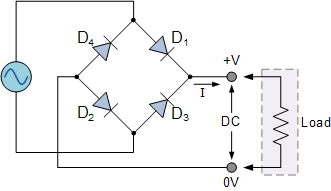
\includegraphics[width=.67\textwidth]{assets/full-wave-rectifier.png}
	\caption{Full-wave rectifier}
	\label{fig:full-wave-rectifier}
\end{figure}
\begin{marginfigure}
	\centering
	\begin{tikzpicture}
		\begin{axis}[
				width=\textwidth,
				xtick={0, 3.14159266, 6.28318531, 9.42477796, 12.566371},ytick={-.5, 0, .5},
				xticklabels={\(0\), \(\lf{T}{2}\), \(T\), \(\lf{3T}{2}\), \(2T\)},yticklabels={\(-I_0\), \(0\), \(I_0\)},
				xlabel=\(t\),ylabel=\(I\),
				ymin=-.6,ymax=.6,
				xmin=0,domain=0:12.7,
				samples=200,axis lines=middle,
			]
			\addplot[jiyopink, ultra thick] {0.5 * sin(deg(x)};
			\addplot[jiyoyellow, ultra thick, smooth] {0.5 * abs(sin(deg(x)};
			\legend{a.c., full-wave};
		\end{axis}
	\end{tikzpicture}
	\caption{Full-wave rectification}
	\label{fig:fwr-graph}
\end{marginfigure}
The effective frequency of the signal is doubled (\cref{fig:fwr-graph}).

\section{Kirchoff's laws (optional)}
\begin{enumerate}
	\item At a circuit junction, current arriving \(=\) current leaving\sidenote{\it{current arriving} as positive, \it{current leaving} as negative}.
	      \[\sum I = 0\]
	\item Around any closed loop, algebraic sum of emf \(=\) algebraic sum of current times resistance\sidenote{\(\epsilon\) and \(I\) are positive starting from the positive terminal}.
	      \[\sum_i \epsilon_i = \sum_i I_iR_i\]
\end{enumerate}

\section{Other examples}
\begin{example}{}{3-capacitors}
	What is the effective capacitance of this system?
	\begin{center}
		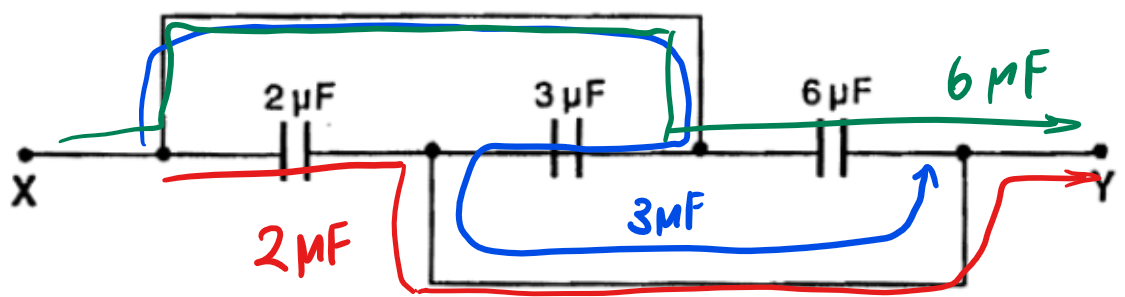
\includegraphics[width=0.7\textwidth]{assets/3-capacitors.png}
	\end{center}
	There are a total of 3 paths from X to Y. On each path,
	we encounter one of the three capacitors \(\implies\) capacitors are in parallel.
	\(C_\text{eff} = 2 + 3 + 6 = \qty{11}{\micro\farad}\).
\end{example}

\begin{example}{}{resistor-network}
	In this network of resistors, what is the p.d.~between X and Y?
	\begin{center}
		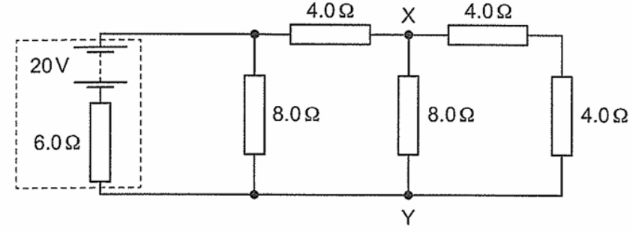
\includegraphics[width=.8\textwidth]{assets/r-network.png}
	\end{center}
	We can group the resistors together:
	\begin{center}
		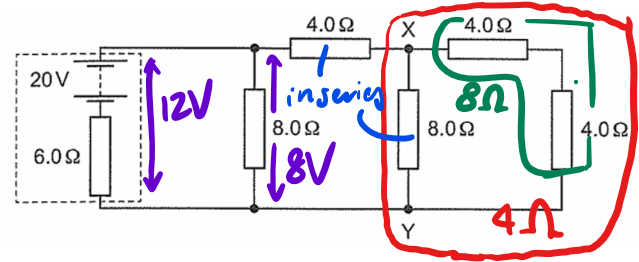
\includegraphics[width=.8\textwidth]{assets/r-network-redraw.png}
	\end{center}
	\begin{itemize}
		\item green: the two \(\qty{4.0}{\ohm}\) resistors combine to form an \(\qty{8}{\ohm}\) resistor
		\item red: combine the new \(\qty{8}{\ohm}\) resistor with the \(\qty{8.0}{\ohm}\) resistor across XY, to get a \(\qty{4}{\ohm}\) resistor
		\item purple: by potential divider, the p.d.~across the jumble of resistors is \(\lf{4}{\ab(4+6)}\cdot 20 = \qty{8}{\volt}\)
		\item blue: by potential divider, the \it{red resistor} and remaining \(\qty{4.0}{\ohm}\) resistor each have a p.d.~across them of \hil{\qty{4}{\volt}}
	\end{itemize}
\end{example}

\begin{example}{}{}
	Another network of resistors. What is the p.d.~between X and Y,
	and which point (X or Y) has greater potential?
	\begin{center}
		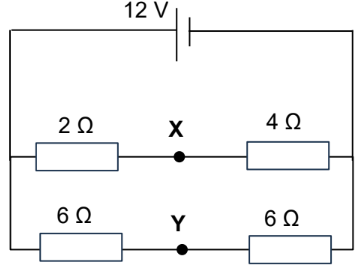
\includegraphics[width=.5\textwidth]{assets/rxy.png}
	\end{center}
	We \underline{start at \qty{0}{\volt} at the negative terminal}!
	\begin{center}
		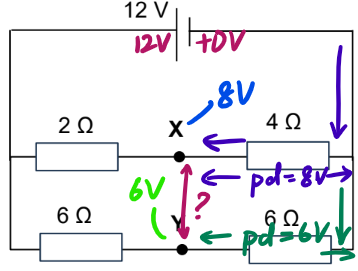
\includegraphics[width=.5\textwidth]{assets/rxy-redraw.png}
	\end{center}
	\begin{align*}
		V_X           & = \lf{4}{\ab(4+2)}\cdot 12=\qty{8}{\volt}\quad\text{(pot.~at a point)}       \\
		V_Y           & = \lf{6}{\ab(2\cdot 6)}\cdot 12= \qty{6}{\volt}\quad\text{(pot.~at a point)} \\
		\Delta V_{XY} & = 8-6=\hil{\qty{2}{\volt}}\quad\text{(p.d.!)}
	\end{align*}
	Point X is at higher potential.
\end{example}

\chapter{Magnetic field}
\section{RHGR}
\bf{Right-hand grip rule} determines the direction of \(I\) from
the direction of \(\va{B}\), and v.v.
\begin{figure}[htpb]
	\centering
	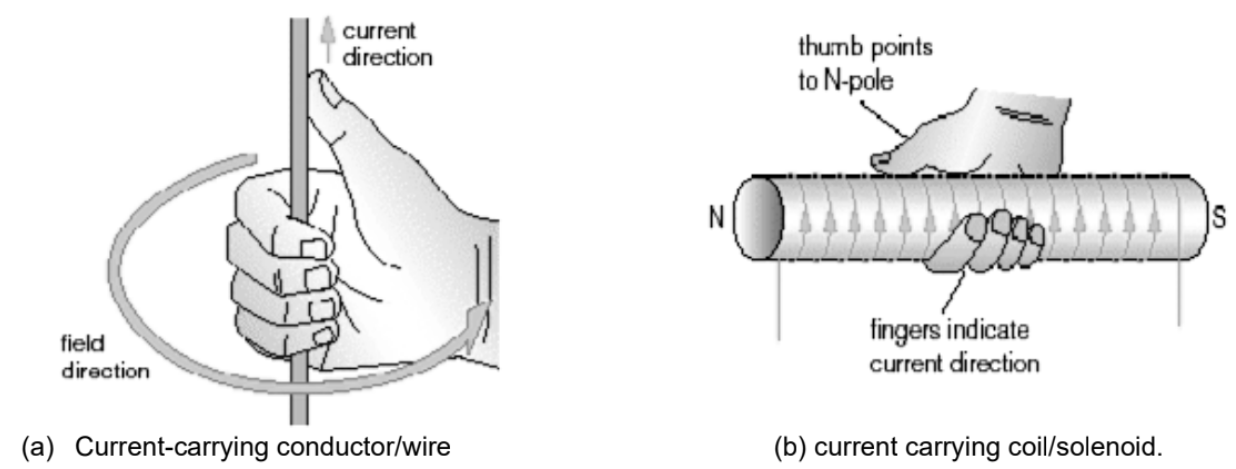
\includegraphics[width=.8\textwidth]{assets/rhgr.png}
	\caption{Right-hand grip rule}
	\label{fig:rhgr}
\end{figure}

Typical field lines (\cref{fig:bfield-lines}):
\begin{figure}[htpb]
	\centering
	\begin{minipage}{.65\textwidth}
		\centering
		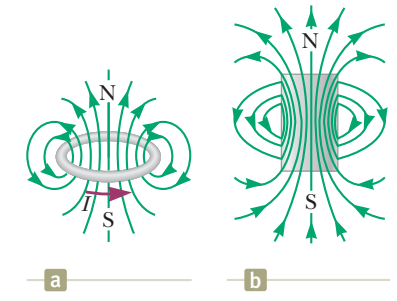
\includegraphics[width=.7\textwidth]{assets/bfields-1.png}
		\caption{Field lines for (a) circular coil and (b) bar magnet}
	\end{minipage}
	\begin{minipage}{.34\textwidth}
		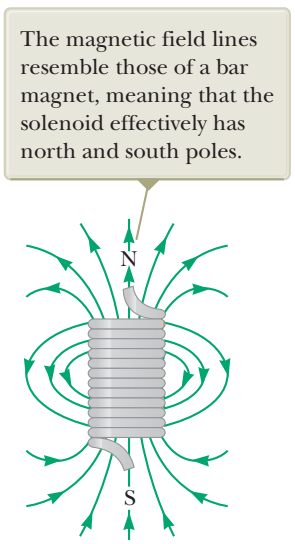
\includegraphics[width=.7\textwidth]{assets/bfields-solenoid.png}
		\caption{Field lines for solenoid}
	\end{minipage}
	\label{fig:bfield-lines}
\end{figure}
The direction of \(\va{B}\) at any point is tangent to the magnetic field line at that point.

\begin{example}{}{ferrous-core}
	For solenoids, inserting a \bf{soft iron core} magnetises the core in the same direction,
	adding to the magnetic flux density \(\implies\) strengthens net magnetic field.
\end{example}

\begin{definition}{Magnetic flux density}{bdensity}
	Force acting \it{per unit current per unit length}
	on a conductor placed perpendicular to a magnetic field [tesla: \unit{\tesla}]
	\\\\
	\footnotesize
	Magnetic flux density is \underline{1 tesla} if force per unit current per unit length
	acting on a conductor placed perpendicular to the \(\va{B}\)-field is \qty{1}{\newton\per\ampere\per\metre}.
\end{definition}

\section{FLHR}
\bf{Fleming's left-hand rule} determines the direction of the
magnetic force \(\va{F}\) from the direction of current
and magnetic field, v.v.
\begin{marginfigure}
	\centering
	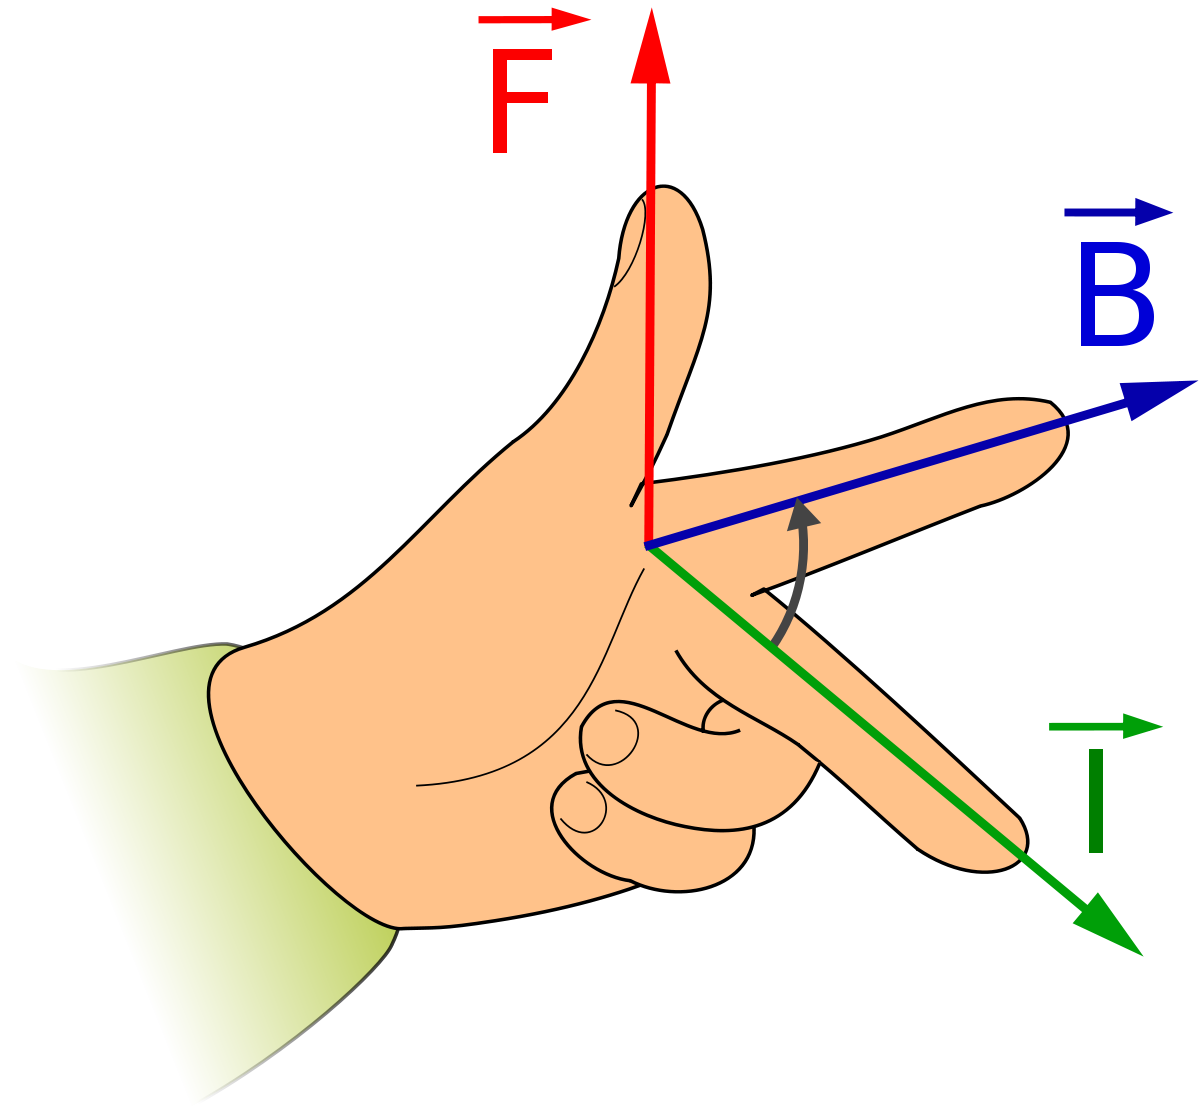
\includegraphics[width=.7\textwidth]{assets/flhr.png}
	\caption{Fleming's left-hand rule}
\end{marginfigure}

The \term{\bf{magnetic force}} acting on a straight conductor of length \(L\) carrying a current \(I\) in a magnetic field
of flux density \(B\) is
\begin{equation*}
	F_B = B_\perp IL
\end{equation*}
where \(B_\perp\) is the component of \(\va{B}\) perpendicular to the conductor.

\subsection{Like currents attract, unlike currents repel}
This is an application of FLHR. Parallel conductors carrying currents
in the \it{same direction} experience an attractive force on each other (by N3L);
currents in the \it{opposite direction} result in a repulsive force on each other (by N3L).
\begin{figure}[htpb]
	\centering
	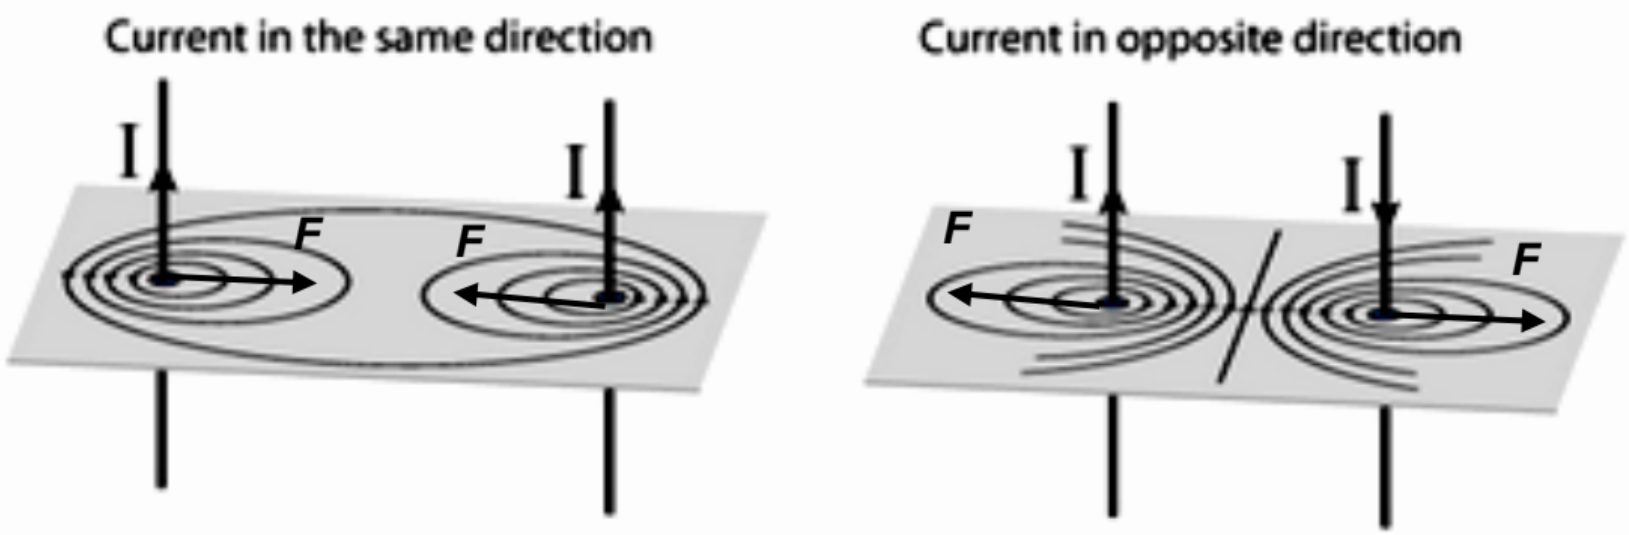
\includegraphics[width=.8\textwidth]{assets/like-unlike-currents.png}
	\caption{Like currents attract, unlike currents repel}
\end{figure}

\subsection{DC motor}
We can determine the direction of \(\va{F}\) on either side of the motor's coil
using FLHR, and hence the direction of rotation.
\begin{marginfigure}
	\centering
	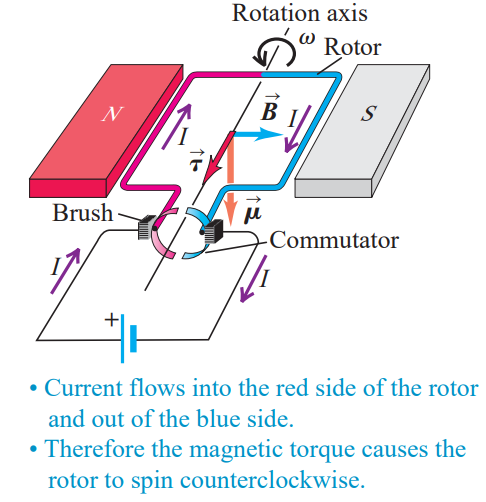
\includegraphics[width=\textwidth]{assets/dc-motor.png}
	\caption{A d.c.~motor}
\end{marginfigure}
Taking the side of the coil parallel to the current to have length \(L\),
and the side of the coil perpendicular to the current to have length \(w\), the magnetic force on each side of the coil is
\[F = nBIL\]
Since the force on the \term{pink} and \textcolor{jiyoblue}{blue} sides is equal, the coil only rotates.
With \(\theta\coloneq \) the angle between the plane of the coil and the magnetic field, the torque on the coil is
\begin{align*}
	\tau\ab(\theta) & = Fd = nBIL\cdot w\sin\theta \\
	\max\tau        & = nBILw
\end{align*}

\section{Moving charge in \(\va{B}\)-field}
\begin{marginfigure}
	\centering
	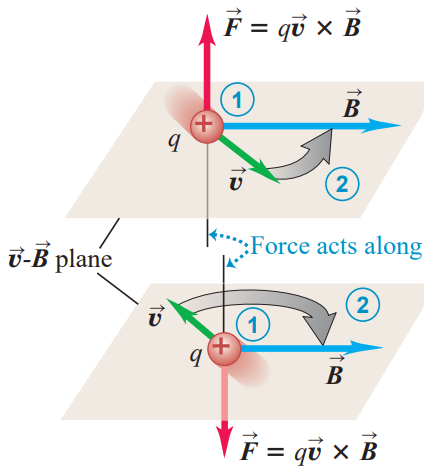
\includegraphics[width=\textwidth]{assets/flhr-moving-q.png}
	\caption{Moving positive charge in \(\va{B}\)-field}
	\label{fig:flhr-moving-q}
\end{marginfigure}
A moving charge \(q\) with velocity \(v\) experiences a magnetic force.
\[F = B_\perp q v\]
A negative charge experiences \(\va{F}\) in the opposite direction.

\begin{marginfigure}
	\centering
	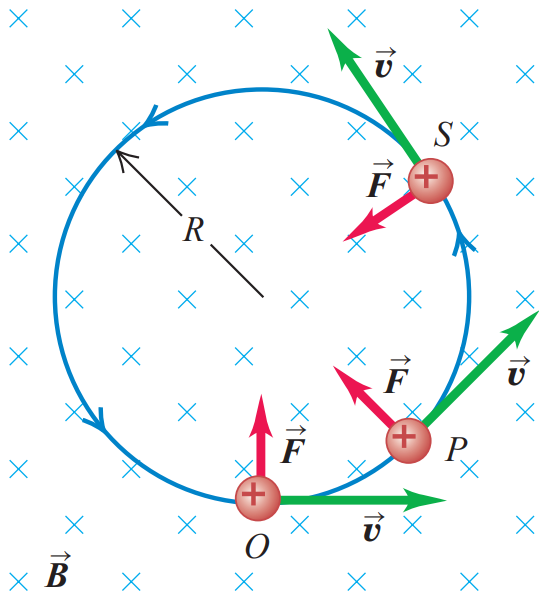
\includegraphics[width=.8\textwidth]{assets/q-circle.png}
	\caption{Moving charge in uniform \(\va{B}\)-field}
	\label{fig:moving-q-circular}
\end{marginfigure}
In a \it{uniform} magnetic field, the magnetic force provides
the charge with centripetal acceleration.
\begin{example}{}{why-constant-v}
	\it{Why does the charge move with constant speed?}

	Magnetic force \(\va{F}\) and the velocity of the charge \(\va{v}\) are always
	perpendicular to each other. Since the magnitudes of \(B\) and \(q\)
	are constant, magnitude of \(v\) is also constant.
\end{example}
\begin{align*}
	Bqv & = \f{mv^2}{r} \\
	r   & = \f{mv}{Bq}
\end{align*}
The charge will continue to trace a circle \it{only} if
the charge enters perpendicular to the field \(\va{v} \perp \va{B}\).

Otherwise, only the perpendicular component of \(\va{v}\), \(v_\perp\), contributes to the magnetic force.
\(v_\parallel\) remains constant, causing the charge to trace a helix.
For a magnetic field \(\va{B} = B\ii\), and a velocity \(\va{v} = v\cos\theta\ii + v\sin\theta\jj\), the radius of the helix is
\begin{align*}
	Bqv_\perp & = \f{m{v_\perp}^2}{r}                       \\
	r         & = \f{mv\sin\theta}{Bq}                      \\
	T         & = \f{2\pi r}{v_\perp} = \f{2\pi m}{Bq}      \\
	p         & = v_\parallel T = \f{2\pi mv\cos\theta}{Bq}
\end{align*}

\subsection{Velocity selector}
\begin{marginfigure}
	\centering
	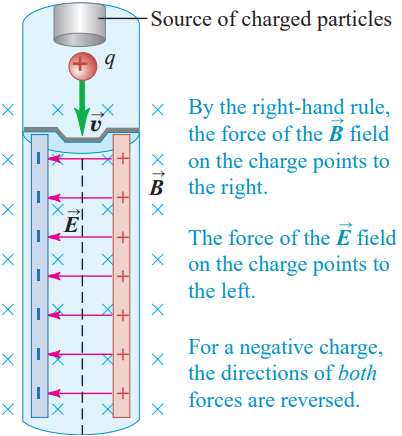
\includegraphics[width=.8\textwidth]{assets/v-selector.png}
	\caption{Velocity selector}
	\label{fig:v-selector}
\end{marginfigure}

Coinciding an \(\va{E}\) field with a \(\va{B}\) field creates a
\term{velocity selector}. For the particle's path to remain undeflected,
\(\va{F}_E = -\va{F}_B\), so
\begin{align*}
	qE & = Bqv      \\
	v  & = \f{E}{B}
\end{align*}

\chapter{Electromagnetic induction}

\section{Definitions}
\begin{marginfigure}
	\centering
	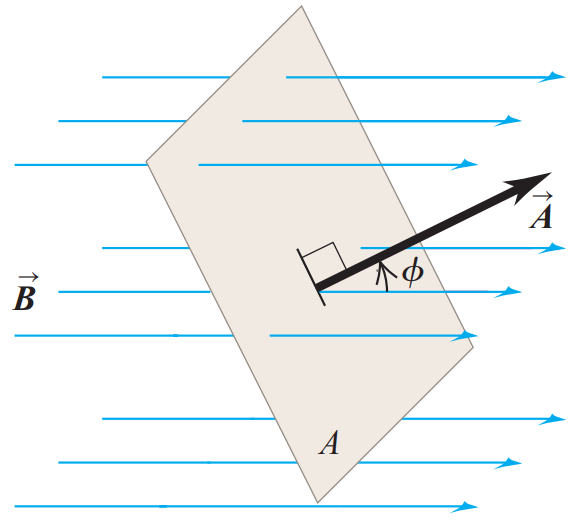
\includegraphics[width=.85\textwidth]{assets/phi-b.png}
	\caption{\(\Phi = B\cdot A\cos\phi = \ab(B\cos\phi) A\)}
	\label{fig:phi-b}
\end{marginfigure}
\begin{definition}{Magnetic flux}{bflux}
	The product of magnetic flux density \(B\) and cross-sectional area \(A_\perp\)
	\it{perpendicular} to the direction of \(B\). [weber: \unit{\weber}]
	\[\Phi = BA_\perp = B_\perp A\]
	\footnotesize
	\qty{1}{\weber} is the magnetic flux through a surface of area \qty{1}{\metre\squared} if a magnetic field
	of flux density \qty{1}{\tesla} is perpendicular to the surface.
\end{definition}

\begin{definition}{Magnetic flux linkage}{bflux-linkage}
	The product of the number of turns and the magnetic flux through each turn.
	\[\Phi_\text{link} = N\Phi\]
\end{definition}

\section{Faraday's law}
\begin{definition}{Faraday's law}{faraday}
	Magnitude of the induced emf \(\mathcal{E}\) is \it{directly proportional}
	to the rate of change of magnetic flux linkage \it{or the rate of cutting of magnetic flux}.
	\[\mathcal{E} = \ab|\odv{\Phi}{t}|\]
\end{definition}

\begin{marginfigure}
	\centering
	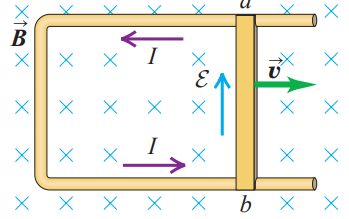
\includegraphics[width=\textwidth]{assets/u-loop.png}
	\caption{Sliding bar}
	\label{fig:u-loop}
\end{marginfigure}

\begin{example}{}{u-loop}
	(\Cref{fig:u-loop}) A conducting bar of length \(L\) slides on two parallel conducting rails in a uniform magnetic field
	\(B\) directed into the page. The bar moves to the right with a constant velocity \(v\). \it{What is the emf induced in the bar?}
	\\
	After a small time interval \(\odif{t}\), the bar moves a horizontal distance \(\odif{s}\).
	In this time, there will be a small change in magnetic flux, \(\odif{\Phi} = B\odif{A} = BL\odif{s}\).
	Since \(\epsilon \propto \odv{\Phi}{t}\),
	\begin{align*}
		\mathcal{E} & = \ab|\odv{\Phi}{t}| \\
		            & = B\ab|\odv{A}{t}|   \\
		            & = BL\ab|\odv{s}{t}|  \\
		            & = BLv
	\end{align*}
\end{example}

\begin{marginfigure}
	\centering
	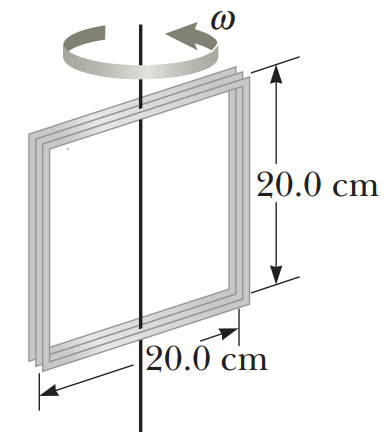
\includegraphics[width=.67\textwidth]{assets/rotating-coil.png}
	\caption{Rotating square loop}
	\label{fig:square-loop}
\end{marginfigure}
\begin{example}{}{rotating-loop}
	(\Cref{fig:square-loop}) A \(N\)-turn square loop of side \(x\) rotates in a uniform magnetic field \(B\)
	with an angular frequency \(\omega\). What is the \it{maximum emf} induced in the loop?
	\\\\
	At any time \(t\), the angle the loop makes with the magnetic field is \(\theta = \omega t\).
	Then the magnetic flux linkage is
	\begin{equation*}
		\Phi = NBA_\perp       = NBx^2\cos\theta  =NBx^2\cos\omega t
	\end{equation*}
	So the induced emf is
	\begin{align*}
		\mathcal{E}      & = \ab|\odv{\Phi}{t}|                \\
		                 & = NBx^2 \ab|\odv{}{t} \cos\omega t| \\
		                 & =  NB\omega x^2\sin\omega t         \\
		\max \mathcal{E} & = NB\omega x^2
	\end{align*}
\end{example}
\begin{marginfigure}
	\centering
	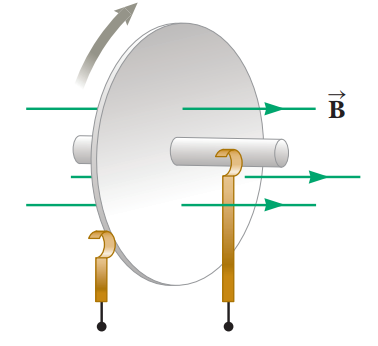
\includegraphics[width=.8\textwidth]{assets/faraday-disk.png}
	\label{fig:faraday-disk}
	\caption{Faraday disk}
\end{marginfigure}

\begin{example}{}{faraday-disk}
	(\Cref{fig:faraday-disk}) A uniform magnetic field \(B\) is passed
	through a rotating conducting disk of radius \(r\) and const.~angular velocity \(\omega\).
	What is the magnitude of the induced emf?

	For a short time \(\odif{t}\), the disk rotates through a small angle \(\odif{\theta} = \omega\odif{t}\) (by definition).
	The small area swept out by the disk in this time is \(\odif{A} = \f{1}{2}r^2\odif{\theta}\).
	Then
	\begin{align*}
		\mathcal{E} & = \ab|\odv{\Phi}{t}|       \\
		            & = B\ab|\odv{A}{t}|         \\
		            & = \f{1}{2}Br^2\dot{\theta} \\
		            & = \f{1}{2}Br^2\omega
	\end{align*}
\end{example}

\section{Lenz's law}
\begin{definition}{Lenz's law}{lenz}
	The polarity of the induced emf is such that the induced current
	creates a magnetic field to \it{oppose the change in magnetic flux}.
	\[\mathcal{E} = -\odv{\Phi}{t}\]
\end{definition}

How to determine \term{direction of induced current}:
\begin{enumerate}
	\item Pick a point of view.
	\item Determine the direction of the change in magnetic flux (increasing/decreasing?).
	\item Flip the direction to get the direction of the induced magnetic field (created by the induced current).
	\item Use RHGR to obtain the direction of the induced current. {\small Induced emf is in this direction too.}
\end{enumerate}

\begin{example}{}{u-loop-2}
	Referring to \cref{fig:u-loop}, what is the direction of induced current?
	\begin{itemize}
		\item As the bar moves \it{rightwards}, there is an increase in magnetic flux \it{rightwards}.
		\item By Lenz's law, increase in magnetic flux induces an emf to create a magnetic field \it{outwards}.
		\item Using RHGR, the direction of the induced current in the rectangular loop formed is \it{anticlockwise}.
	\end{itemize}
\end{example}
\begin{marginfigure}
	\centering
	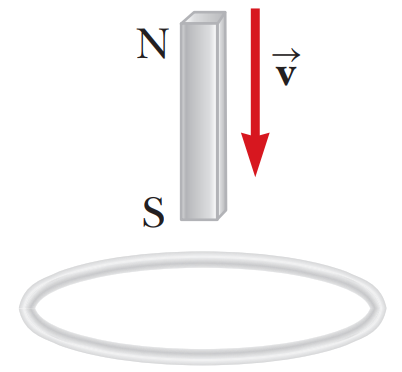
\includegraphics[width=.67\textwidth]{assets/falling-magnet.png}
	\caption{Falling magnet under gravity}
	\label{fig:falling-magnet}
\end{marginfigure}
\begin{example}{}{falling-magnet}
	Referring to \cref{fig:falling-magnet}, what is the direction of induced current?
	\vspace*{1em}
	When the magnet enters the loop,
	\begin{itemize}
		\item there is increasing upward flux (since \(\va{B}\) of bar magnet points upwards).
		\item By Lenz's law, the induced emf creates a magnetic field to oppose the flux change, so the \it{induced magnetic field is downwards}.
		\item By RHGR, \it{induced current is clockwise}.
	\end{itemize}
	As the magnet continues falling, the magnet accelerates (due to gravity).
	\begin{itemize}
		\item Upward magnetic flux continues to increase, since the velocity of the magnet increases.
		\item By Lenz's law, the induced emf creates a magnetic field to oppose the flux change, so the \it{induced magnetic field is downwards}.
		\item By RHGR, \it{induced current is clockwise}, and \it{of an increasing magnitude}.
		\item Induced emf \it{increases in magnitude}.
	\end{itemize}
	\vspace*{.5em}
	At the instant where the magnet leaves,
	\begin{itemize}
		\item there is a sudden decrease in upward magnetic flux.
		\item By Lenz's law, the induced emf creates a magnetic field to oppose the flux change, so the \it{induced magnetic field is upwards}.
		\item By RHGR, \it{induced current is anticlockwise}.
	\end{itemize}
\end{example}

\section{Eddy currents}
Eddy currents form when the magnetic flux varies periodically (e.g.~through an alternating current, or mechanical oscillation).
\begin{marginfigure}
	\centering
	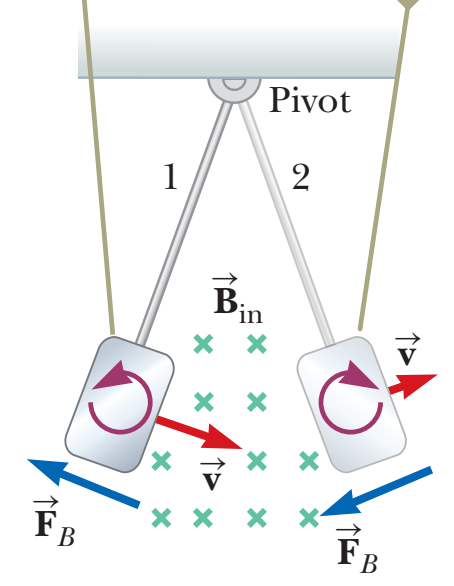
\includegraphics[width=.8\textwidth]{assets/eddy-current.png}
	\caption{Eddy currents}
	\label{fig:eddy-current}
\end{marginfigure}
We can \bf{reduce eddy currents} by laminating conducting components (building up in thin layers).
Increased resistance \(\implies\) reduced eddy currents \(\implies\) reduced energy loss due to eddy currents.

\section{Transformers}
\it{Ideal transformers} have coils of \it{zero resistance}.
\[\lf{V_s}{V_p} = \lf{N_s}{N_p}\]

\begin{marginfigure}
	\centering
	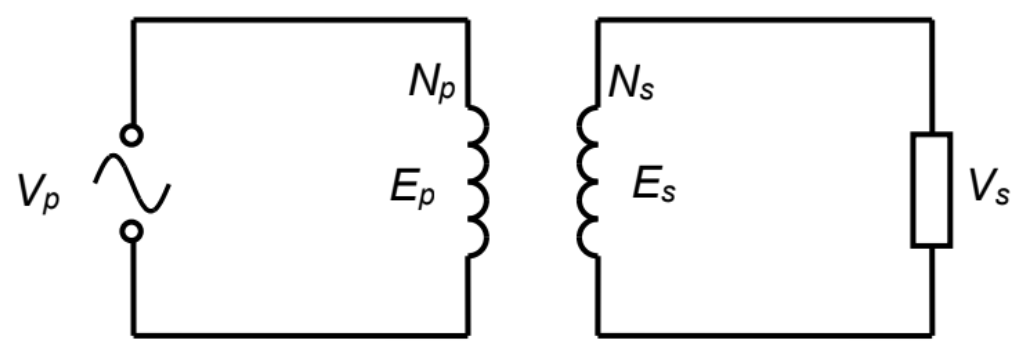
\includegraphics[width=\textwidth]{assets/transformer.png}
	\caption{Transformer}
	\label{fig:transformer}
\end{marginfigure}

In an ideal situation, the transformers are also \qty{100}{\percent} efficient:
\begin{align*}
	P_p     & = P_s     \\
	V_p I_p & = V_s I_s
\end{align*}
If the transformer is not ideal, then calculate \(P_\text{out}\) from \(P_\text{in}\)
given \(\eta\).

\hil{Eddy currents} can be reduced by \it{laminating the transformer core}
\(\implies\) increased resistance \(\implies\) reduced eddy currents \(\implies\) reduced
energy loss (thermal) \(\implies\) better efficiency.

\hil{Hysteresis} is energy loss resulting from direction of a.c.~periodically reversing.
It causes heating in the core. Hysteresis can be reduced by using \it{soft iron core}
or \it{alloys}.

\chapter{Quantum physics}
\section{Photoelectric effect}
\begin{definition}{Photoelectric effect}{photoelectric}
	Phenomenon in which (photo)electrons are liberated from a \it{cool metal surface}
	when \it{e.m.~radiation} of sufficiently high frequency is incident on it.
\end{definition}
\begin{definition}{Work function}{work-func}
	\(\phi\), minimum amount of energy required to remove an electron from the metal surface.
	\vspace*{.5em}
	\footnotesize This property is intrinsic to the metal.
\end{definition}
\begin{definition}{Threshold frequency}{f-naught}
	\(f_0\), minimum frequency of the electromagnetic radiation
	required to liberate photoelectrons from a metal surface.
	\[\phi = hf_0\]
\end{definition}

Electromagnetic radiation exists in quanta---\term{photons}:
\begin{definition}{Photon}{photon}
	A discrete packet or \it{quantum} of energy of e.m.~radiation. Its energy \(E\) is
	\[E = hf = \lf{hc}{\lambda}\]
\end{definition}

Each photon--electron interaction is \it{one-to-one}: energy of one photon
is either fully absorbed by one electron, or not at all.

The photoelectric effect proves that light is quantised, by observing:
\begin{itemize}
	\item electrons emitted iff \(f_\text{incident} \geq f_0\) (threshold frequency), regardless of intensity
	\item maximum k.e.~of emitted electrons \(\propto\) frequency of incident light, regardless of intensity
	\item maximum k.e.~of emitted electrons independent of intensity of incident light
	      \[K_{\max}= h f_{\text{photon}} - \phi\]
	\item rate of emission of photoelectrons \(\propto\) intensity of incident light
	      \[\text{intensity}\times\text{area} = P = \f{E}{t} = \f{n_{\ce{e-}}}{t}\times{hf}\]
\end{itemize}

\section{Diffraction and interference}
\begin{marginfigure}
	\centering
	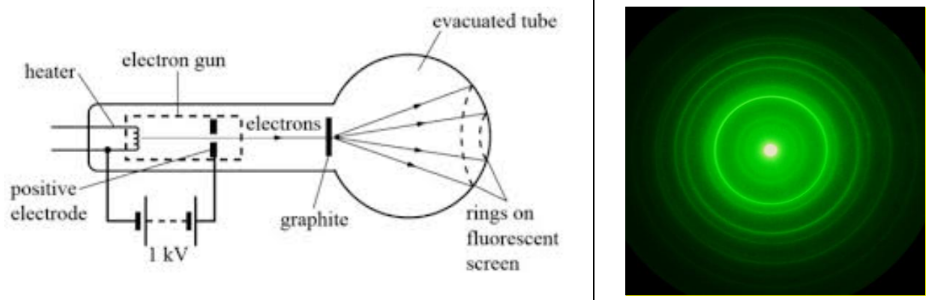
\includegraphics[width=\textwidth]{assets/e-diffraction.png}
	\caption{Diffraction experiment; diffraction pattern of \ce{e-}}
	\label{fig:e-diffraction}
\end{marginfigure}
The diffraction pattern of an electron beam contains
\it{concentric rings} with \it{alternating bright and dark regions}.

\(\implies \)\hil{\ce{e-} exhibit wave-like behaviour.}

As such, the electrons must be associated with a \it{wavelength}, with
the same order of magnitude as the crystal's atomic spacing.

\(\implies\) \hil{\ce{e-} in motion have an associated \(\lambda\).}

\begin{marginfigure}
	\centering
	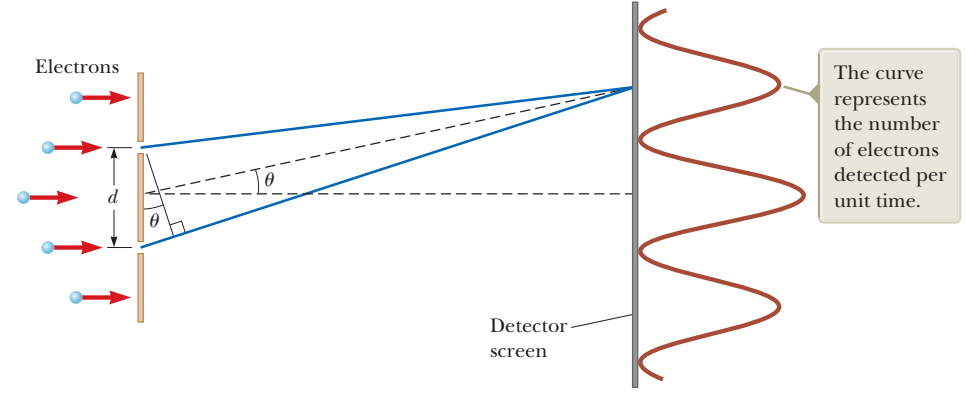
\includegraphics[width=\textwidth]{assets/e-double-slit.png}
	\caption{Double slit experiment}
	\label{fig:e-double-slit}
\end{marginfigure}
Over time, the accumulated detections form a pattern
resembling Young's double slit. High \ce{e-} density regions
correspond to \it{constructive interference}; low \ce{e-} density
regions correspond to \it{destructive interference}.

\(\implies\) \hil{\ce{e-} possess wave-like properties.}

\begin{definition}{Wave-particle duality}{wp-duality}
	The principle that \it{neither the wave or particle model alone} is sufficient
	to describe microscopic systems.
	\\\footnotesize
	Both e.m.~radiation and matter exhibit \it{wave-like and particle-like behaviour}.
\end{definition}

Photons have \term{momentum}, which can be associated with its de Broglie \term{wavelength}.
\[p = \f{E}{c} = \f{h}{\lambda}\]
\hil{Wave-like behaviour is due to a particle's motion}.

\section{Wave-like behaviour}
The \term{wavefunction} \(\psi\ab(x)\) describes the waveform
formed by matter/radiation. It must satisfy the conditions:
\begin{itemize}
	\item \(\psi\ab(x)\) must be continuous and oscillatory
	\item \(\psi\ab(x)\) must be normalisable, s.t.~\(\int_{-\infty}^{+\infty} {\ab|\psi\ab(x)|}^2 \odif{x}=1\)
	\item \(\psi\ab(x)\to 0\) as \(x\to\pm\infty\), total probability must be finite
\end{itemize}

\begin{definition}{Probability density function}{pdf}
	The probability of finding a particle (e.g.~electron, photon) at a position \(x\).
	It is the square of the amplitude of the wavefunction.
	\[\text{pdf} \coloneq {\ab|\psi\ab(x)|}^2\]
\end{definition}

The probability of finding a particle within a region of width \(\Delta x\) is then \(\text{proba} = {\ab|\psi\ab(x)|}^2\cdot\Delta x\).

The probability of finding a particle within a region \(a\leq x\leq b\) is
\[\int_a^b {\ab|\psi\ab(x)|}^2\odif{x}\]

\section{Heisenberg uncertainty principle}
\begin{definition}{Heisenberg uncertainty principle}{heisenberg}
	\[\Delta x \Delta p_x \geq h\]
	A particle's position and momentum cannot both be sharply defined.
\end{definition}

For a wave packet to be \it{localised} in position (i.e.~confined within a certain \(\Delta x\)),
waves of a large range of wavelengths \(\Delta\lambda\) must be superposed.
Spread in \(\lambda\) \(\implies\) spread in \(p\), by \(p=\lf{h}{\lambda}\).

For a wave packet have a perfectly defined \(\lambda\) (i.e.~perfectly defined \(p\)),
it must be a single infinite wave extending over space (i.e.~\it{delocalised}), hence
\(\Delta x\) is large.

\section{Quantisation of energy}
\subsection{Particle-in-box}
\begin{marginfigure}
	\centering
	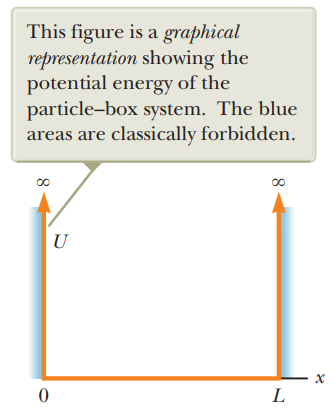
\includegraphics[width=0.75\textwidth]{assets/particle-in-box-u.png}
	\caption{\(U\ab(x)\) for particle in box}
	\label{fig:particle-in-box-u}
\end{marginfigure}
Confine a particle that only possesses k.e.~\(K\) in a box
spanning \(0\leq x\leq L\). Since the particle has no potential energy,
\begin{equation*}
	U\ab(x) = \begin{cases}
		0      & 0\leq x \leq L   \\
		\infty & \text{otherwise}
	\end{cases}
\end{equation*}
Whatever wavefunction \(\psi\ab(x)\) the particle follows must satisfy \it{boundary conditions}, since
it cannot be found outside the box:
\[\psi\ab(x=0)=0,\quad\psi\ab(x=L)=0\]

Since the particle is \it{free}, it can form \it{stationary waves} in the box. For the standing wave
to fit exactly in the box, the box must contain an integer number of segments (length \(\lf{\lambda}{2}\)):
\[L=\lf{n\lambda}{2} \implies \lambda_n = \lf{2L}{n}\]
\hil{The particle can only take on \it{allowed wavelengths}.}

\begin{figure}[htpb]
	\centering
	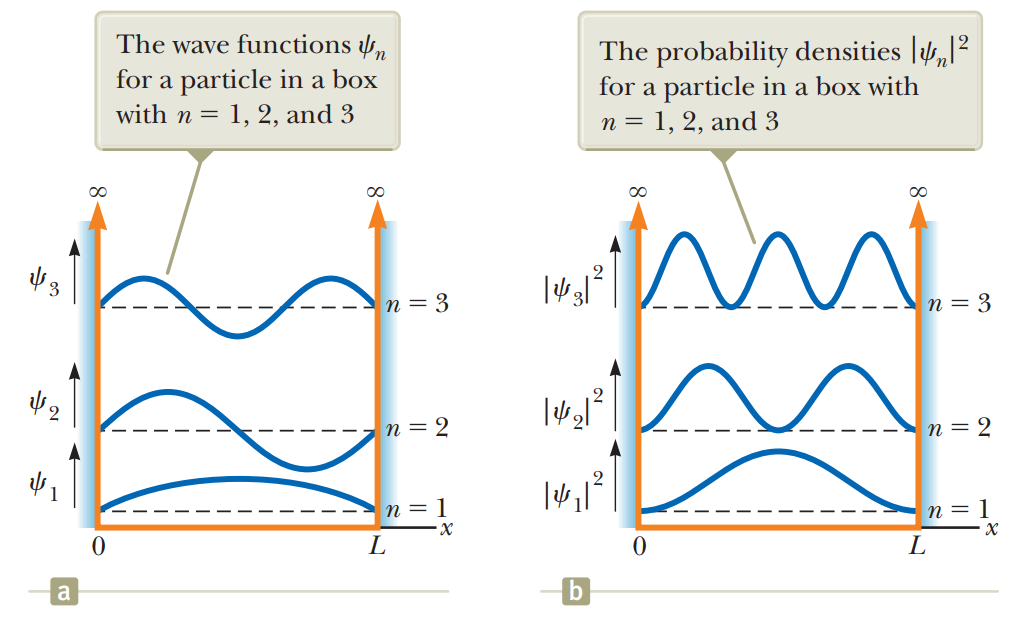
\includegraphics[width=0.75\textwidth]{assets/psi-in-box.png}
	\caption{\(\psi\) and \({\ab|\psi|}^2\) for particle in box}
	\label{fig:psi-in-box}
\end{figure}
This also means that the particle can only take on \it{allowed momenta}:
\[p_n = \f{h}{\lambda_n} = \f{nh}{2L}\]

\begin{marginfigure}
	\centering
	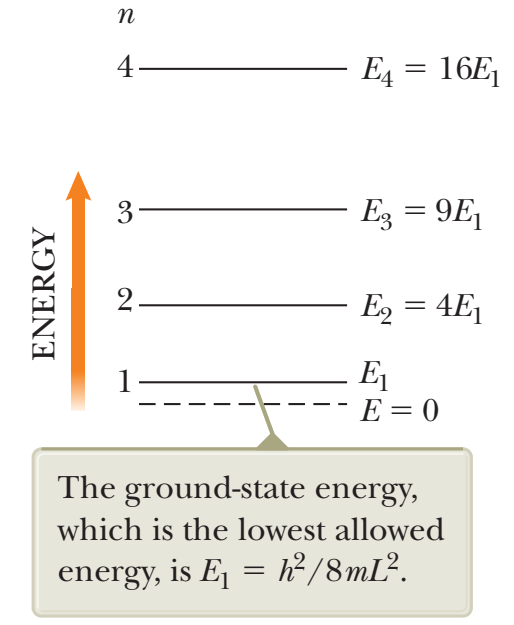
\includegraphics[width=.8\textwidth]{assets/energy-levels.png}
	\caption{Allowed energy levels}
	\label{fig:energy-levels}
\end{marginfigure}
And therefore, the particle can only take on \it{allowed energies}, which are quantised:
\[E_n = K_n = \f{p_n^2}{2m} = \f{n^2h^2}{8mL^2}\]

Electrons can transition between any two energy levels, so
the number of \it{allowed transitions} is \({}^nC_2\) for \(n\) energy levels.

\begin{definition}{Ground state}{ground-state}
	The lowest possible energy state of the atom, where \(n = 1\).
\end{definition}

\section{Line spectra}

\begin{definition}{Excitation}{excitation}
	The absorption of a photon by one \ce{e-} to promote
	the electron from a lower allowed energy level to a higher allowed energy level.
	\[hf = E_\text{hi} - E_\text{lo}\]
\end{definition}
\(\therefore\;\) The energy of the photon must be \it{exactly} the energy
difference \(\Delta E\).

Light may be emitted by atoms when electrons de-excite.
The light is not observed as a continuous spectrum of wavelengths,
but appears as a series of discrete lines at specific wavelengths.
\begin{definition}{De-excitation}{deexcitation}
	The release of energy by one \ce{e-} \it{in the form of a photon}
	when it moves from a higher energy level to a lower energy level.
	\[hf = E_\text{hi} - E_\text{lo}\]
\end{definition}

\begin{definition}{Ionisation}{ionisation}
	The absorption of sufficient energy by an electron
	to completely leave the atom.
\end{definition}

\subsection{Emission spectra}
\begin{marginfigure}
	\centering
	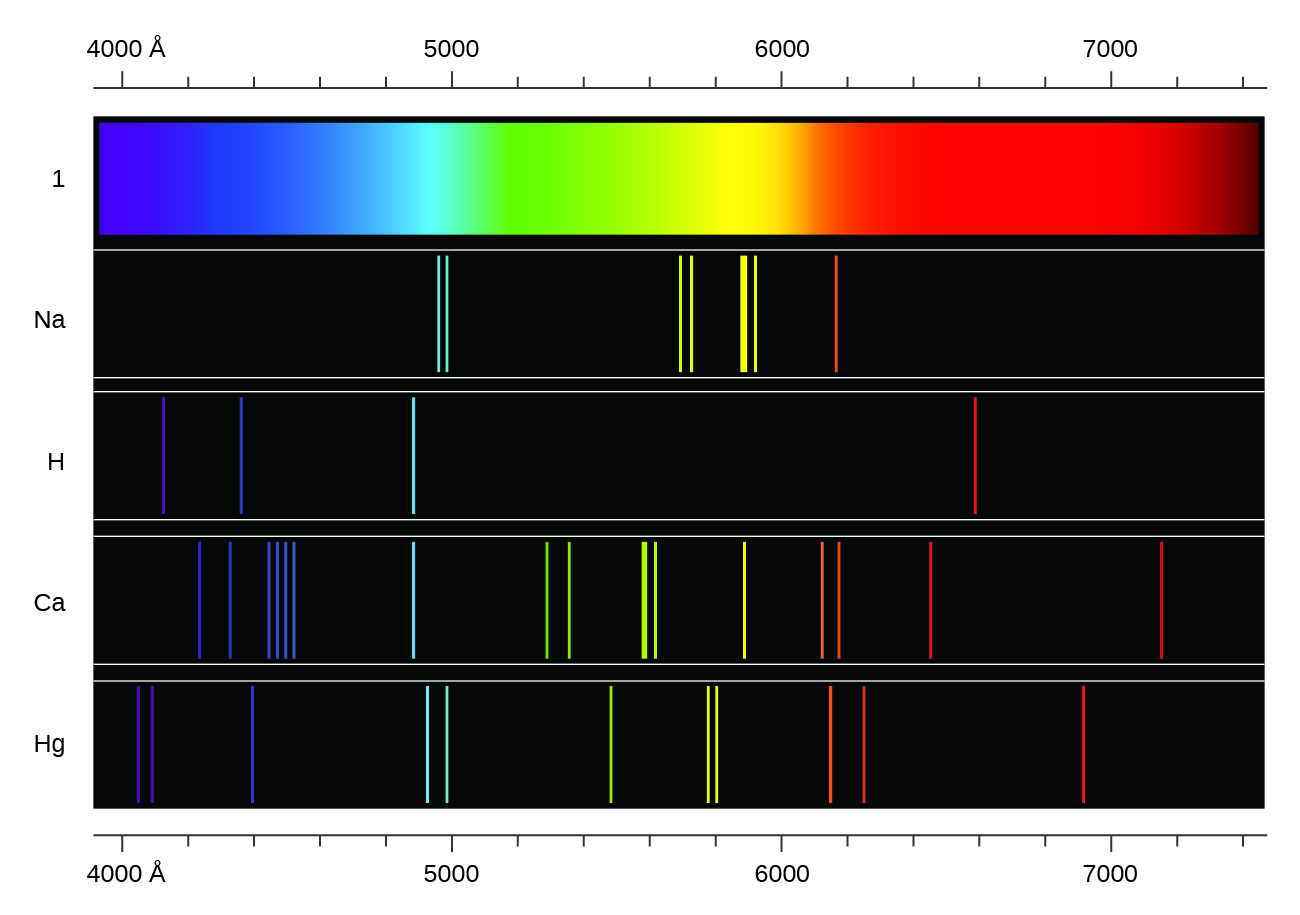
\includegraphics[width=\textwidth]{assets/atomic-spectra.jpg}
	\caption{Emission spectra of \ce{Na}, \ce{H}, \ce{Ca} and \ce{Hg}}
	\label{fig:emission-spectra}
\end{marginfigure}
When e.m.~radiation is incident on atoms, \ce{e-} can become excited.

Atoms collide with fast-moving electrons in a discharge tube,
causing part of the free electrons' k.e.~to be transferred to the atoms.
The \it{bound electrons} in the atoms excite.

When the excited atoms de-excite, the bound electrons return to a lower
energy level and each emit one photon.
\[hf = E_{\text{photon}} = E_\text{hi} - E_\text{lo}\]
This produces emission spectra (\cref{fig:emission-spectra}).

\subsection{Absorption line spectra}
Light of a \it{continuous spectrum} of wavelengths passes through a
\underline{cool gas} at \underline{low pressure}.

Photons whose energies match the energy difference
between ground state and an excited state are absorbed;
these photons are removed from the light.

\begin{marginfigure}
	\centering
	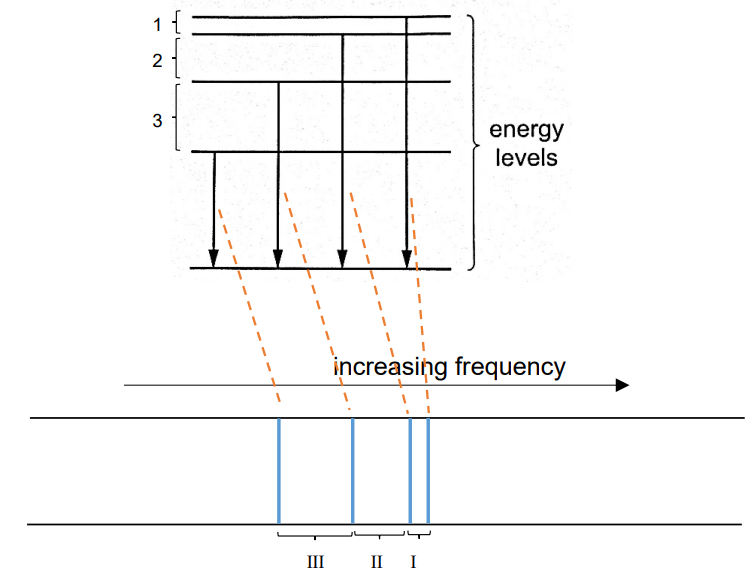
\includegraphics[width=\textwidth]{assets/absorption-spectra.png}
	\caption{Absorption line spectrum}
	\label{fig:absorption-spectra}
\end{marginfigure}
Although the atoms in the gas release photons
when they eventually de-excite,
\begin{itemize}
	\item the \it{released photons are radiated in all directions}; they may not reach the observer
	\item de-excitation may happen through \it{intermediate transitions}, so the emitted photons may have different energies from the original incident photons.
\end{itemize}
The resultant intensity of these select photons decreases \(\implies\)
appear as dark lines.
Since \(\Delta E \propto f\), the spacing between lines
is proportional to the energy gap involved in allowed transitions.

\chapter{Nuclear physics}
\section{Atomic structure}
\begin{marginfigure}
	\centering
	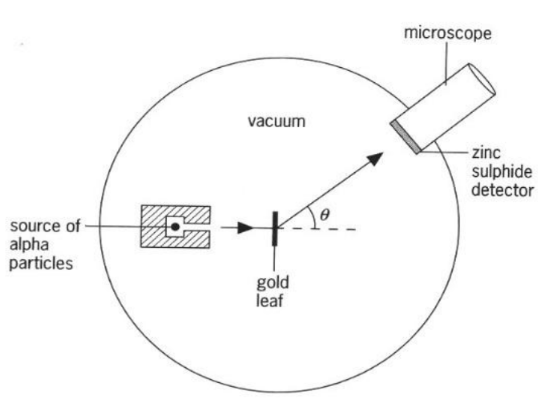
\includegraphics[width=\textwidth]{assets/rutherford-setup.png}
	\caption{Setup of Rutherford scattering}
	\label{fig:rutherford-setup}
\end{marginfigure}
\bf{Why is the vacuum necessary?} \(\alpha\) particles
only travel short distances in air.

Conclusions of Rutherford gold foil experiment:
\begin{marginfigure}
	\centering
	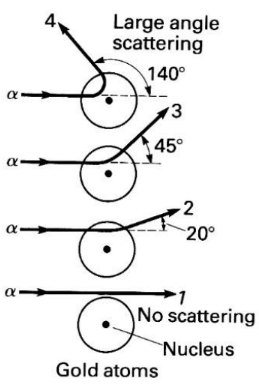
\includegraphics[width=.5\textwidth]{assets/rutherford-scattering.png}
	\caption{Scattering of \(\alpha\) particles}
	\label{fig:rutherford-scattering}
\end{marginfigure}
\begin{itemize}
	\item Large proportion of \(\alpha\) particles are undeflected \(\implies\) most of the atom is empty space
	\item Some \(\alpha\) particles are deflected at small angles \(\implies\) all positive charge and mass is concentrated in a very small volume (the \term{nucleus}!)
	\item Very small proportion of \(\alpha\) particles are deflected at angles more than \qty{90}{\degree} \(\implies\) the nucleus is very small compared to the atom
\end{itemize}

\section{Nuclear reactions}
In nuclear reactions, these must be \it{conserved}:
\begin{itemize}
	\item sum of proton numbers
	\item sum of nucleon numbers
	\item net charge
	\item total momentum\sidenote{for 2 products, momenta are equal in magnitude and opposite in direction!}
	\item total mass--energy
\end{itemize}

Nuclear force is \bf{short-range} and \bf{attractive}, and
falls to 0 at distances greater than \qty{1.5}{\femto\meter}.
\begin{definition}{Binding energy of a nucleus}{binding-energy}
	Energy required to separate the nucleus
	into its consituent free nucleons.
	\\
	{\footnotesize Also equal to energy released when free nucleons are bound together in a nucleus!}
\end{definition}

\begin{definition}{Binding energy per nucleon}{binding-energy-per-nucleon}
	Average energy required to remove a nucleon from the nucleus.
	\\
	{\footnotesize Greater binding energy per nucleon \(\implies\) more stable nucleus!}
\end{definition}

To find \bf{binding energy}, where \(Z\) is the proton number and \(N\) is the neutron number:
\begin{align*}
	\text{binding energy} = E & = \ab(\Delta m)c^2                                \\
	                          & = \ab[\ab(Zm_p + Nm_n) - m_{\text{nucleus}})] c^2
\end{align*}

To find \bf{energy change} of reaction,
\begin{align*}
	\Delta E & = \ab(\sum m_{\text{reactants}} - \sum m_{\text{products}}) c^2        \\
	         & = \sum \text{BE}_{\text{products}} - \sum \text{BE}_{\text{reactants}}
\end{align*}
If the energy change is \it{positive}, energy is released.\sidenote{If no radiation is emitted, released energy is the products' k.e.}
If the energy change is \it{negative}, energy must be supplied (e.g.~through the k.e.~of the reactants) for the reaction to take place.

\section{Radioactivity}
Radioactivity is \bf{spontaneous} and \bf{random}.
\begin{definition}{Spontaneity}{spontaneity}
	Radioactivity is not triggered by external factors/influences;
	rate of decay is unaffected by environmental conditions (e.g.~temperature, pressure).
\end{definition}

\begin{definition}{Randomness}{randomness}
	Impossible to predict which nucleus decays next, or when a particular nucleus will decay.
\end{definition}
Randomness is evidenced by fluctuations in the count rate.

\subsection{Decay types}
A few types of decay in \cref{tab:decay-types}.
\begin{table}[htpb]
	\centering
	\begin{tabular}{r p{0.25\textwidth} p{0.25\textwidth} p{0.25\textwidth}}
		\toprule
		                  & alpha                                                      & beta                                                           & gamma                               \\
		\midrule
		nature of decay   & \(\ce{^4_2He}\) nucleus                                    & \(\ce{^0_{-1}e}\)                                              & photon                              \\
		charge            & \(+2e\)                                                    & \(-e\)                                                         & \(0\)                               \\
		mass              & \qty{4}{\atomicmassunit}                                   & \(m_e\)                                                        & \(0\)                               \\
		penetrating power & easily stopped by paper/skin/a few \unit{\centi\metre} air & stopped by \qty{1}{\metre} air / \qty{3}{\milli\metre} \ce{Al} & several \unit{\centi\metre} \ce{Pb} \\
		\bottomrule
	\end{tabular}
	\caption{Types of decay}
	\label{tab:decay-types}
\end{table}

\begin{itemize}
	\item In \bf{alpha decay}, released energy shows up as the k.e.~of the alpha particle and
	      daughter nucleus. \it{The products have momenta equal in magnitude and opposite in direction.}
	\item In \bf{beta-minus decay}, a neutron in the nucleus transforms into 1 proton and
	      1 electron \ce{^0_{-1}e}; the electron is ejected with some k.e. The remaining k.e.~is
	      present in an \it{antineutrino} \(\bar{\nu}\).
	\item In \bf{beta-plus decay}, a proton in the nucleus transforms into 1 neutron and
	      1 \it{positron} \ce{^0_{+1}e} (charge: \(+e\)). The remaining k.e.~is
	      present in a \it{neutrino} \(\nu\).
\end{itemize}

\section{Measuring decay}
\begin{definition}{Activity}{activity}
	Number of disintegrations per unit time. [\unit{\becquerel} = {\small 1 disintegration \unit{\per\second}}]

	Where \(N \coloneq\) number of radioactive nuclei present,
	\[A = -\odv{N}{t}\]
\end{definition}
Activity cannot be directly measured, so count rate \(C\) is used as a proxy.
\[C \propto A\]
\it{Subtract background count rate} before doing any calculations.

\begin{definition}{Decay constant}{decay-constant}
	The probability per unit time that a nucleus will decay.
	\[R = R_0\exp\ab(-\lambda t)\qquad\text{where}\:R=N, C, A\]
\end{definition}

\begin{definition}{Half-life}{half-life}
	\begin{itemize}
		\item Average time taken for \it{half} the original number of nuclei in a sample to decay \underline{or}
		\item Average time for sample's activity to reduce to \it{half} its original value
	\end{itemize}
	\[t_{\lf{1}{2}} = \f{\ln 2}{\lambda}\]
\end{definition}

\end{document}
